%
%  PARA TRABALLOS EN GALLEGO USAR (LINEA 12): \usepackage[galician]{babel}
%  PARA TRABALLOS EN CASTELLANO USAR (LINEA 13): \usepackage[spanish]{babel}
%
% Para los acentos usamos codificacion UTF-8 (LINEA 10): \usepackage[utf8]{inputenc} 
% Si se usase la codificacion es_ES.ISO-8859-1 (LINEA 11): \usepackage[latin1]{inputenc}
% La conversion de acentos se hace con: iconv -f UTF-8 -t ISO-8859-1 filename.tex
%
% Como se incluyen figuras eps hay que compilar con: latex traballo , dvipdf traballo
%

\documentclass[12pt,twoside,a4paper]{book}
% pódense engadir todos os packages necesarios
\usepackage[utf8]{inputenc}
% \usepackage[latin1]{inputenc}
\usepackage[galician]{babel}
% \usepackage[spanish]{babel}
\usepackage{graphicx}
\usepackage[dvips]{epsfig}
\usepackage{amssymb}
\usepackage{eurosym}
\usepackage{float}
\usepackage{latexsym}
\usepackage{a4}
\usepackage{listings}
% \usepackage{hyperref} % menús no pdf pero non leva ben co package galician

\begin{document}
\pagestyle{empty}
\begin{center}
{\bf\Large UNIVERSIDADE DE SANTIAGO DE COMPOSTELA}

\vspace{0.5cm}

\includegraphics[width=5cm]{figuras/logo_usc.eps}

\vspace{0.5cm}
{\bf\large ESCOLA TÉCNICA SUPERIOR DE ENXEÑARÍA}

\vspace{2cm}
{\bf\LARGE Título do Traballo de Fin de Grao}

\vspace{0.5cm}
{\bf\LARGE Subtítulo do Traballo de Fin de Grao}
\end{center}

\vspace{2cm}
\hspace{4cm}\begin{tabular}{l}
{\it\Large Autor:} \\
{\bf\Large Martín Coego Pérez} \\
~ \\
{\it\Large Directores:} \\
{\bf\Large Paulo Félix Lamas} \\
{\bf\Large Tomás Teijeiro Campo} \\
\end{tabular}

\vspace{2cm}
\begin{center}
{\bf\Large Grao en Enxeñaría Informática}

\vspace{0.5cm}
{\bf\large Febreiro 2011}

\vspace{0.5cm}
Traballo de Fin de Grao presentado na Escola Técnica Superior de Enxeñaría da Universidade de Santiago de Compostela para a obtención do Grao en Enxeñaría Informática
\end{center}


\cleardoublepage
\pagestyle{plain}
\pagenumbering{roman}

\includegraphics[width=4cm]{figuras/logo_usc.eps}

\vspace{1cm}
{\bf D. Paulo Félix Lamas}, Profesor do Departamento de Electrónica e
Computación da Universidade de Santiago de Compostela, e {\bf D. Tomás Teijeiro
Campo}, membro do Departamento de Electrónica e Computación da Universidade de
Santiago de Compostela,

\vspace{1cm}
INFORMAN:

\vspace{1cm}
Que a presente memoria, titulada {\it Deseño dunha linguaxe orientada ao xogo de
rol en liña}, presentada por {\bf D.
Martín Coego Pérez} para superar os créditos correspondentes ao
Traballo de Fin de Grao da titulación de Grao en Enxeñaría Informática,
realizouse baixo a nosa dirección no Departamento de Electrónica e Computación
da Universidade de Santiago de Compostela.

\vspace{1cm}
E para que así conste aos efectos oportunos, expiden o presente informe en
Santiago de Compostela, a 8 de febreiro do 2017:

\vspace{2cm}
\begin{tabular}{lll}
O director, & O codirector, & O alumno, \\
~ \\
~ \\
~ \\
~ \\
~ \\
~ \\
~ \\
Paulo Félix Lamas & Tomás Teijeiro Campo & Martín Coego Pérez
\end{tabular}

 % paxina de certificación (optativa)
\cleardoublepage
\pagestyle{plain}
\chapter*{Agradecementos}
Se se quere pór algún agradecemento, este vai aquí.

 % paxina de agradecementos (optativa) 
\cleardoublepage
\pagestyle{plain}
\chapter*{Resumo}
Se se quere pór resumo, este vai aquí.

 % páxina de resumo (optativa) 

\cleardoublepage
\pagestyle{plain}
\tableofcontents
\listoffigures
\listoftables

% Agora incluimos os capítulos. Cambiamos a numeración e as cabeceiras
\cleardoublepage
\pagenumbering{arabic}
\setcounter{page}{1}
\pagestyle{headings}
\chapter{Introdución}
\hyphenation{In-te-re-se}

Introdución: composta por Obxectivos Xerais, Relación da Documentación que conforma a Memoria, Descrición do Sistema, Información Adicional de Interese (métodos, técnicas ou arquitecturas utilizadas, xustificación da súa elección, etc.).

\cleardoublepage
\chapter{Xestión do proxecto}

% Planificación e presupostos: debe incluír a estimación do costo (presuposto) e
% dos recursos necesarios para efectuar a implantación do Traballo, xunto coa
% planificación temporal do mesmo e a división en fases e tarefas. Recoméndase
% diferenciar os costos relativos a persoal dos relativos a outros gastos como
% instalacións e equipos.

A xestión de proxectos conleva unha serie de metodoloxías e técnicas encamiñadas
a planificar temporalmente o proxecto para acadar o seu alcance no prazo
previsto, así como garantir a calidade do produto final. Neste capítulo
definirase a metodoloxía de desenvolvemento empregada no proxecto, e farase unha
estimación de prazos e custos.

\section{Metodoloxía de desenvolvemento}
Unha das decisións máis importantes que se deben tomar ao comezo do proxecto é a
metodoloxía de desenvolvemento a empregar. Esta metodoloxía debe permitirnos
estruturar o traballo para garantir a súa finalización cuns mínimos
de calidade aceptables.
\par
A escolla da metodoloxía fundaméntase nas características do proxecto. neste
caso concreto, o noso programa ten unha temática pouco explorada no
mercado, e empregará diversas tecnoloxías e recursos relativamente novos para o
desenvolvedor. A maiores, este ten unha experiencia reducida na xestión de
proxectos grandes. Tendo todas estas cuestións en conta, parece apropiado optar
por unha metodoloxía de desenvolvemento áxil e descartar o uso de metodoloxías
menos tolerantes ao cambio.

\subsection{Scrum}
Optouse polo emprego de \textit{Scrum}\cite{scrum} para o desenvolvemento do
software.
En Scrum, o desenvolvemento realízase de forma incremental mediante iteracións:
as tarefas distribúense temporalmente en sprints de unha ou dúas semanas por
norma xeral. Poténciase especialmente a interacción co cliente e márcanse uns
prazos fixos para cumprir obxectivos, para o cal é preciso priorizar os
requisitos regularmente.

\subsubsection{Actividades}
No modelo de Scrum as reunións xiran en torno aos sprints, e podemos atopar as
seguintes actividades:
\begin{itemize}
  \item Daily Scrum ou Stand-up Meeting: Reunións diarias nas que se revisa o
  o estado do proxecto por parte do equipo. Neste caso concreto non son
  relevantes por ser un proxecto dunha soa persoa.
  \item Sprint Planning Meeting: Reunión de planificación do sprint. Realízase
  ao inicio do sprint, e nela estipúlase o traballo que se realizará no mesmo.
  \item Sprint Review Meeting: Reunión de revisión do sprint. Faise ao final do
  sprint, e revísase o traballo completado e non completado.
  \item Sprint Retrospective: Na retrospectiva do sprint, os membros do equipo
  dan as súas impresións sobre o mesmo. Isto ten a finalidade de mellorar o
  proceso de forma continuada.
\end{itemize}

\subsection{Ferramentas de xestión empregadas}
Hai numerosas ferramentas dispoñibles para xestionar proxectos de tipo Scrum.
Neste proxecto empregarase Acunote, que permite levar o control da lista de
requisitos e dos sprints coas súas tarefas.

\subsubsection{Acunote}
Trátase dunha ferramenta web que ofrece distintas funcionalidades enfocadas na
xestión de proxectos con metodoloxías Scrum, tales como a creación e mantemento
dunha lista de requisitos priorizada ou \textit{product backlog} para o
proxecto, xestión de sprints (con nome, data de inicio e fin, e tarefas) e, xa
dentro de cada sprint, o control do estado de cada tarefa, incluído o tempo
investido nela e o tempo total requerido. A maiores, Acunote ofrece gráficas e
estatísticas do proceso xeradas automaticamente para levar o control do mesmo.

\section{Planificación temporal}
A planificación temporal desenvolveuse inicialmente en base ao anteproxecto
existente. A metodoloxía Scrum non ofrece unha estruturación concreta do
proxecto en fases de vida debido ao seu carácter iterativo, mais pódese facer
unha aproximación dunha división de etapas do mesmo segundo o tipo de traballo
desenvolvido en cada unha delas.

\subsection{Fase inicial}
Nesta primeira fase desenvolveuse unha descrición extensa do proxecto e das
funcionalidades que o produto resultante debe ofrecer. Dividiuse o programa en
compoñentes e determinouse a forma de interactuar destes entre si. Ademais
disto, tomáronse as decisións necesarias sobre a organización do traballo e a
xestión da documentación e de versións.

\subsection{Fase de análise}
A principal tarefa desta fase foi a de realizar unha análise de requisitos a
partir de distintas historias de usuario. Definíronse os conceptos chave do
sistema de forma máis precisa, e marcáronse formalmente os requisitos e as
limitacións do software. Tamén se decidiron as principais tecnoloxías a
empregar no software.

\subsection{Fase de definición da linguaxe}
Esta fase estivo centrada no desenvolvemento dunha definición formal da linguaxe
do xogo, a linguaxe {\it COE}, e a súa implementación en Java. Non se inclúe o
desenvolvemento do analizador semántico, tarefa que forma parte da seguinte
fase.

\subsection{Fase de desenvolvemento}
Na fase de desenvolvemento implementáronse os distintos compoñentes software do
proxecto coas súas distintas funcionalidades. Trátase da fase máis longa, e a
súa realización documéntase en maior detalle no capítulo \ref{ch:implementacion}
pertinente deste documento.

\subsection{Fase de probas}
Nesta última fase fanse probas unitarias do sistema. A maiores, o sistema
instálase nun servidor web para realizar probas con usuarios que poden ser
útiles para extraer posibles melloras en usabilidade ou detectar erros. 

\section{Xestión da configuración}
Os elementos de configuración son os distintos elementos cos que traballamos no
proxecto, dos cales precisamos manter un control
sobre os cambios que se poidan realizar neles, xa que poden afectar
sensiblemente ao desenvolvemento do propio proxecto.
\par
Xa que estamos a falar dun proxecto exclusivamente de desenvolvemento de
software, será o propio código fonte o que consideraremos elemento de
configuración. Para manter a súa integridade e realizar o control de cambios
empregaremos a ferramenta Git.

\subsection{Git}
Git \cite{git} é un software de control de versións que nos permite estabelecer
repositorios de software e controlar os cambios que se realizan no código. Con
Git podemos crear un repositorio para cada elemento independente do proxecto e
manter un control dende calquera ordenador no que traballemos. Permite tamén
visualizar os cambios realizados en cada {\it submit} e desfacelos en caso de
ser preciso.
\subsubsection{GitHub}
GitHub é unha ferramenta web para desenvolvedores que ofrece aloxamento gratuíto
para repositorios Git. Deste modo, é posible manter o repositorio en liña e
traballar co mesmo dende distintos equipos sen necesidade de configurar un
servidor web.

\section{Análise de custos}
Os custos deste proxecto recaen principalmente na man de obra, os equipos
informáticos e os servidores. Non hai custos adicionais en adquirir paquetes de
software, xa que un dos requisitos especificados dende o principio é o uso
exclusivo de ferramentas libres.
\par
O servidor empregado é un VPS \footnote{VPS: Virtual Private Server. É un
servidor virtual dentro dunha máquina real. Habitualmente é ofrecido por
empresas de hosting como unha alternativa barata aos servidores dedicados.}
contratado cunha empresa, que empregaremos para instalar o noso software e facer
probas de usuario.
Calcúlase que transcorrerán 2 meses dende o momento no que é contratado ata a
exposición do proxecto.
\par
Adicionalmente, consideramos un 20\% de custos indirectos.

\begin{tabular} { | c c r | r | }
\hline
Item & Cantidade & Custo unitario & Custo total \\
\hline
PC & 1 & 1000,00 \euro{} & 1000,00 \euro{} \\
\hline
Persoal & 412,5 horas & 15,00 \euro{} & 6187,50 \euro{} \\
\hline
VPS & 2 meses & 20 \euro{} & 40 \euro{} \\
\hline
& & Subtotal: & 7227,50 \euro{} \\
\hline
&& Custos indirectos: & +20\% \\
\hline
&& Total: & 8673 \euro{} \\
\hline
\end{tabular}
\cleardoublepage
\chapter{Análise}

Antes de comezar a desenvolver o software deberase facer unha especificación dos
requisitos que este debe cumprir. Neste caso o primeiro que faremos será definir
casos de uso do sistema, para posteriormente extraer a partir deles unha serie
de requisitos funcionais e non funcionais.

\section{Definicións}
Nos casos de uso e requisitos faremos referencia a estas definicións, polo que é
necesario explicalas aquí con precisión.

\subsubsection{Partida}
Instancia concreta deste software xestionada por un administrador. Cada partida
debe ter unha base de datos propia e un directorio cos ficheiros que compoñen o
mundo. Non se contempla a comunicación entre partidas distintas.

\subsubsection{Mundo}
O mundo de xogo é a abstracción de todos os obxectos e clases correspondentes a
unha partida. Pódese distinguir entre a definición do mundo e o seu estado:
\begin{itemize}
\item Definición: O conxunto das clases descritas polos directores de xogo.
\item Estado: O conxunto dos obxectos instanciados a partir das clases.
\end{itemize}

\subsubsection{Xogador}
Usuario que ten control dun personaxe e toma decisións en base a este. Os
xogadores non poden modificar o mundo directamente, senón que as súas
interaccións co mundo realízanse a través dos personaxes.

\subsubsection{Director de xogo (DX)}
Usuario con privilexios que pode alterar o mundo de forma directa, e resolver as
decisións dos xogadores. Poden tanto alterar a definición do mundo (creando e
modificando clases) como cambiar o estado do mesmo (instanciando obxectos e
modificándoos). Os directores de xogo non teñen personaxe propio.

\subsubsection{Clase}
No ámbito do mundo de xogo, abstracción dun conxunto de obxectos con atributos e
métodos comúns, seguindo o paradigma da programación orientada a obxectos. Os
directores de xogo poden crear e modificar estas clases.
\par
Un exemplo de clase sería {\it espada}, {\it porta}, {\it cabalo} ou {\it
guerreiro}.

\subsubsection{Obxecto}
No ámbito do mundo de xogo, cada unha das instancias dunha clase concreta. Os
obxectos {\it existen} no mundo, e sitúanse nun determinad escenario. É labor
dos directores de xogo crealos, modificalos e destruílos. Todos os obxectos
posúen un identificador global dentro do mundo.
\par
Un exemplo de obxecto sería {\it a segunda mesa da posada}, {\it o personaxe dun
dos xogadores} ou {\it o can que acompaña ao grupo de personaxes}.

\subsubsection{Personaxe}
Obxecto especial que representa a un xogador no mundo. Toda a información
percibida polo personaxe será posta en coñecemento do xogador correspondente, e
toda decisión tomada polo xogador determinará as accións do personaxe.

\subsubsection{Decisión}
Descrición verbal dun xogador explicando a acción que pretende que realice o seu
personaxe. As decisións están redactadas en linguaxe informal, pero con
suficiente información como para que o director de xogo poda entender o que o
xogador pretende. É labor do director de xogo xerar as accións a partir das
decisións dos xogadores.
\par
Un exemplo de decisión sería: {\it ''O meu personaxe achégase á espada
incrustada na pedra, di en voz alta 'alá vou' e trata de arrincala.''}

\subsubsection{Acción}
Conxunto de liñas de código que alterarán o mundo de xogo en función dunha
decisión dun xogador. A acción é redactada por un director de xogo segundo o que
interprete lendo a decisión correspondente.

\subsubsection{Suceso}
Conxunto de liñas de código que alterarán o mundo de xogo pero que non depende
da decisión de ningún xogador. Os sucesos son provocados polos directores de
xogo cando precisen alterar algo do mundo sen ser consecuencia directa das
accións dos xogadores.

\subsubsection{Rolda}
No mundo de xogo, en cada escenario as accións se resolven divididas por roldas.
Por cada rolda, cada personaxe pode facer como máximo unha acción. Estas roldas
representan simbolicamente o paso do tempo dentro do mundo, aínda que o avance
do tempo pode non coincidir exactamente en todos as escenarios por igual.

\subsubsection{Rexistro de personaxe}
Todo o que perciba un personaxe determinado será almacenado nun rexistro. O
xogador ten acceso a este rexistro, polo que poderá consultar en todo momento
todo o que o seu personaxe puido oír, ver ou percibir de calquera xeito.

\subsubsection{Escenario}
Cada un dos recintos pechados nos que se divide o mundo de xogo. Tamén coñecidos
como {\it habitacións} ou {\it estancias} noutros sistemas semellantes. Todos os
obxectos están situados nun escenario, incluídos os personaxes, e en calquera
momento poden cambiar de escenario. Os escenarios pódense agrupar en {\it
rexións} mediante nomes compostos.
\par
Exemplos de escenarios poderían ser {\it Capital/mercado}, {\it montañas/mina
abandonada/terceira sección} ou {\it castelo antigo/segunda planta/habitación
1}.

\subsubsection{Tirada}
Resultado aleatorio que representa unha tirada de dados. A tirada especifica o
número de dados tirados e o número de caras de cada dado. Este resultado
emprégase xeralmente para determinar o éxito ou o fracaso das accións dos
personaxes ou doutros obxectos.

\subsubsection{Recipiente}
Calquera obxecto coa capacidade de almacenar outros obxectos. Estes últimos
estarán vinculados ao obxecto recipiente, por tanto atoparanse sempre no mesmo
escenario. Un obxecto pode ser recipiente de varias listas distintas.
Un exemplo de recipiente é {\it un cofre do tesouro}, {\it un barril} ou un {\it
xogador co seu inventario}. Un exemplo de recipiente con varias listas pode ser
{\it un xogador no que se diferencien os obxectos que leva nas mans dos que leva
nas costas}.


\section{Casos de uso}
Mediante os casos de uso podemos representar situacións típicas do noso
software, as cales suporán un bo xeito de extraer requisitos funcionais.

\subsection{Descrición de actores}
Inicialmente teremos que definir os actores que se relacionan co sistema nos
nosos casos de uso. Identificamos tres actores diferenciados: director de xogo,
xogador e administrador.
\begin{itemize}
\item {\bf Director de xogo:} Este actor correspóndese coa definición descrita previamente; o seu cometido por tanto será dirixir a partida, recibindo decisións dos xogadores e transcribíndoas como accións dos seus personaxes.
\item {\bf Xogador:} Calquera usuario que participe na partida cun personaxe. Redacta decisións e envíaas ao DX.
\item {\bf Administrador:} Usuario especial que crea a partida e se encarga de administrala. As súas principais funcións será a asignación do rango de DX a outros usuarios, e a configuración básica da partida.
\end{itemize}

\subsection{Descrición de casos de uso}
A continuación atopamos os seguintes casos de uso, elaborados a partir de
entrevistas con usuarios potenciais. Son posibles situacións que se poden dar
durante a execución do software.
Por simplificar daremos por feito que todos os casos de uso requerirán ao
usuario en cuestión estar autenticado (salvo o caso de uso CU-01).

\subsubsection{CU-01: Alta de xogadores}
\paragraph{Actores}
Xogador
\paragraph{Escenario principal}
O caso de uso comeza cando un usuario anónimo se rexistra no sistema. Para isto
emprega a opción {\it crear novo usuario}, onde introducirá os datos básicos da
súa conta. Por defecto, o seu rol no sistema será o de xogador.

\subsubsection{CU-02: Xestión de usuarios}
\paragraph{Actores}
Administrador
\paragraph{Escenario principal}
O caso de uso comeza cando o administrador desexa asignar un usuario como DX.
Neste caso, abre a sección de {\it xestión de usuarios} e escribe o nome do
usuario cuxos permisos desexa cambiar. O administrador cambia entón o seu tipo
de usuario de {\it xogador} a {\it director de xogo}. De ter xa un personaxe
asignado, deixará de estalo neste mesmo momento.


\subsubsection{CU-03: Definición dunha nova clase}
\paragraph{Actores}
Director de xogo
\paragraph{Escenario principal}
O caso de uso comeza cando un director de xogo pretende crear unha nova clase na
partida. Na interface gráfica deberá acoder á sección de {\it definición do
mundo}. Unha vez aí, escollerá a opción de crear unha clase nova, e implementará
a clase como desexe. Unha vez rematada, o sistema analizará a clase para
comprobar se ten algún erro (léxico ou sintáctico), e en caso de non atopar
ningún, a clase será almacenada e estará lista para o seu uso posterior.

\paragraph{Escenario alternativo}
A clase ten algún erro, por tanto o sistema non a garda nun ficheiro e, no seu
lugar, mostra unha mensaxe de erro instando ao DX a reescribila.

\subsubsection{CU-04: Creación de personaxe}
\paragraph{Actores}
Director de xogo, xogador
\paragraph{Escenario principal}
O caso de uso comeza cando un xogador desexa crear o seu personaxe. O xogador
accede á sección de {\it creación de personaxe}, onde atopará un cadro de texto
que lle solicitará unha breve descrición do que desexa. O xogador redacta o
texto e envíao ao sistema.
\par
O director de xogo trata este texto como unha decisión máis, e a acción
consecuente é crear un obxecto personaxe ligado ao xogador que o solicitou,
situado nun escenario concreta.

\paragraph{Escenario alternativo}
O DX non ten información suficiente na descrición como para facer un personaxe.
O DX elimina esta descrición e escribe unha resposta ao xogador, que se verá
obrigado a repetir o proceso.

\subsubsection{CU-05: Resolución de decisións en accións}
\paragraph{Actores}
Director de xogo, xogador
\paragraph{Escenario principal}
O caso de uso comeza cun xogador desexando facer algo na partida. Accede á
sección de {\it actuar}, onde poderá ler as últimas accións que sucederon no
escenario no que se atopa o seu personaxe. O xogador redacta a súa decisión e
envíaa ao DX. Unha vez feito isto, non poderá tomar máis decisións ata que a
primeira se resolva.
\par
O director de xogo recibe unha notificación de que hai escenarios con decisións
non resoltas. Accese á sección de {\it resolver accións}, onde ve unha lista de
escenarios con decisións sen resolver. Abre un dos escenarios e le a lista de
decisións e os xogadores que as enviaron, ademais do estado actual do escenario.
En consecuencia, escribirá as accións que mellor representen as decisións
tomadas polos xogadores, que pasarán a ser executada polo sistema. Finaliza o
proceso, e o sistema executa o código das accións introducidas polo DX. O
xogador observa entón un breve texto describindo o sucedido.

\paragraph{Escenario alternativo}
O DX comete algún erro escribindo o código das accións, polo que non se poderán
executar. O sistema devolve unha mensaxe de erro.

\subsubsection{CU-06: Creación dun escenario}
\paragraph{Actores}
Director de xogo
\paragraph{Escenario principal}
O caso de uso comeza cando o director de xogo pretende engadir un novo
escenario ao mundo. Accede á sección de {\it lista de escenarios}, onde
aparecerán os escenarios que xa existen debidamente ordenados. Mediante a opción
{\it crear novo escenario} poderá crear un escenario novo de cero (sen
obxectos).
Finaliza o proceso e o escenario créase.

\paragraph{Escenario alternativo}
O DX pode optar por crear o escenario a partir dun modelo e non dende cero.
Neste caso, executarase un código determinado no momento de crearse o escenario,
que a encherá de obxectos predefinidos.

\subsubsection{CU-07: Execución dun suceso}
\paragraph{Actores}
Director de xogo
\paragraph{Escenario principal}
O caso de uso comeza cando o director de xogo pretende causar un suceso nun
escenario. O DX accede á sección de {\it lista de escenarios}, e selecciona o
escenario na que desexe causar o suceso. Unha vez no panel do escenario,
selecciona a opción {\it causar suceso}, e escribe o código do suceso. Cando
finaliza a opción, o sistema executa o código.

\paragraph{Escenario alternativo}
O DX comete algún erro escribindo o código do suceso, polo que non se poderán
executar. O sistema devolve unha mensaxe de erro.

\subsubsection{CU-08: Cambio de escenario dun obxecto}
\paragraph{Actores}
Director de xogo
\paragraph{Escenario principal}
O caso de uso comeza cando o director de xogo pretende mover un obxecto dun
escenario a outro, sexa como consecuencia dunha decisión dun xogador ou non. O
DX escribe o código do cambio de escenario, especificando o obxecto que se
desprazará e o escenario de destino. Cando se executa a acción, o obxecto
abandona o escenario de orixe e pasa a estar no escenario de destino. No momento
de resolver as accións do escenario de destino, o sistema avisará da entrada de
novos obxectos no mesmo para que o DX o teña en conta.


\section{Requisitos funcionais}
\subsubsection{Requisito FN.01}~\\
{\bf Título:} Alta de usuarios\\
{\bf Descrición:} A aplicación debe permitir que se creen novas contas de usuario.\\
{\bf Casos de uso relacionados:} CU-01\\
{\bf Importancia:} Esencial

\subsubsection{Requisito FN.02}~\\
{\bf Título:} Modificación de usuarios\\
{\bf Descrición:} A aplicación debe permitir que se modifiquen contas de usuario
existentes.\\
{\bf Casos de uso relacionados:} CU-02\\
{\bf Importancia:} Esencial

\subsubsection{Requisito FN.03}~\\
{\bf Título:} Identificación de usuarios\\
{\bf Descrición:} A aplicación debe permitir que os usuarios se identifiquen
correctamente.\\
{\bf Casos de uso relacionados:} CU-02, CU-03, CU-04, CU-05, CU-06, CU-07, CU-08\\
{\bf Importancia:} Esencial

\subsubsection{Requisito FN.04}~\\
{\bf Título:} Creación de clases\\
{\bf Descrición:} A aplicación debe permitir ao director de xogo crear clases
novas no mundo.\\
{\bf Casos de uso relacionados:} CU-03\\
{\bf Importancia:} Esencial

\subsubsection{Requisito FN.05}~\\
{\bf Título:} Modificación de clases
{\bf Descrición:} A aplicación debe permitir ao director de xogo modificar
clases existentes.\\
{\bf Casos de uso relacionados:} CU-03\\
{\bf Importancia:} Esencial

\subsubsection{Requisito FN.06}~\\
{\bf Título:} Eliminación de clases\\
{\bf Descrición:} A aplicación debe permitir ao director de xogo eliminar clases
existentes. A aplicación debe garantir que non se borra unha clase da que hai
obxectos instanciados.\\
{\bf Casos de uso relacionados:} CU-03\\
{\bf Importancia:} Esencial

\subsubsection{Requisito FN.04}~\\
{\bf Título:} Herdanza de clases\\
{\bf Descrición:} A aplicación debe permitir facer que unhas clases sexan
fillas de outras, herdando deste xeito os seus métodos.\\
{\bf Casos de uso relacionados:} CU-03\\
{\bf Importancia:} Esencial

\subsubsection{Requisito FN.07}~\\
{\bf Título:} Creación de obxecto\\
{\bf Descrición:} A aplicación debe permitir crear novos obxectos dende as
clases xa existentes. Estes obxectos créanse no contexto dun escenario
determinado.\\
{\bf Casos de uso relacionados:} CU-04, CU-05, CU-06, CU-07
{\bf Importancia:} Esencial

\subsubsection{Requisito FN.08}~\\
{\bf Título:} Modificación de obxecto\\
{\bf Descrición:} A aplicación debe permitir modificar os atributos de obxectos existentes.\\
{\bf Casos de uso relacionados:} CU-05, CU-07
{\bf Importancia:} Esencial

\subsubsection{Requisito FN.09}~\\
{\bf Título:} Eliminación de obxecto\\
{\bf Descrición:} A aplicación debe permitir eliminar obxectos nos escenarios.\\
{\bf Casos de uso relacionados:} CU-05, CU-07
{\bf Importancia:} Esencial

\subsubsection{Requisito FN.10}~\\
{\bf Título:} Ligazón de obxecto personaxe a xogador\\
{\bf Descrición:} A aplicación debe permitir que un determinado obxecto
personaxe se asocie a un xogador, para deste xeito permitir ao xogador ver os
resultados das súas accións e enviar as súas decisións á estancia axeitada.\\
{\bf Casos de uso relacionados:} CU-04\\
{\bf Importancia:} Esencial

\subsubsection{Requisito FN.11}~\\
{\bf Título:} Creación dun escenario baleiro\\
{\bf Descrición:} A aplicación debe permitir ao director de xogo crear un novo
escenario de cero que non conteña obxectos.\\
{\bf Casos de uso relacionados:} CU-06\\
{\bf Importancia:} Esencial

\subsubsection{Requisito FN.12}~\\
{\bf Título:} Eliminación dun escenario\\
{\bf Descrición:} A aplicación debe permitir ao director de xogo eliminar un
escenario do mundo. Todos os obxectos que conteña o escenario serán eliminados.
O escenario non pode conter personaxes.\\
{\bf Casos de uso relacionados:} CU-06\\
{\bf Importancia:} Opcional

\subsubsection{Requisito FN.13}~\\
{\bf Título:} Creación dun modelo de escenario\\
{\bf Descrición:} A aplicación debe permitir ao director de xogo deseñar un
modelo de escenario. Este modelo conterá código que se executará no momento de
crear a estancia.\\
{\bf Casos de uso relacionados:} CU-06\\
{\bf Importancia:} Opcional

\subsubsection{Requisito FN.14}~\\
{\bf Título:} Creación dun escenario dende modelo
{\bf Descrición:} A aplicación debe permitir ao director de xogo crear un novo
escenario empregando un modelo de escenario, executando o código que este modelo contén.\\
{\bf Casos de uso relacionados:} CU-06\\
{\bf Importancia:} Opcional

\subsubsection{Requisito FN.15}~\\
{\bf Título:} Cambio de escenario dun obxecto\\
{\bf Descrición:} A aplicación debe permitir ao director de xogo mover un
obxecto dun escenario a outro. O identificador global do obxecto permanece
igual, pero no novo escenario pode ter un identificador local diferente.\\
{\bf Casos de uso relacionados:} CU-05, CU-07\\
{\bf Importancia:} Esencial

\subsubsection{Requisito FN.16}~\\
{\bf Título:} Envío de decisións\\
{\bf Descrición:} A aplicación debe permitir aos xogadores enviar as súas
decisións para que o DX poda tratalas.\\
{\bf Casos de uso relacionados:} CU-05\\
{\bf Importancia:} Esencial

\subsubsection{Requisito FN.17}~\\
{\bf Título:} Visualización de resultados\\
{\bf Descrición:} A aplicación debe permitir que os xogadores podan ver os
resultados das accións que involucren aos seus personaxes, sexan accións
causadas polas súas decisións, ou accións e sucesos no escenario na que se atopa
o seu personaxe.
{\bf Casos de uso relacionados:} CU-05, CU-07
{\bf Importancia:} Esencial



\section{Restricións de deseño}

\subsubsection{Requisito RD.01}~\\
{\bf Título:} Uso de ferramentas libres\\
{\bf Descrición:} A aplicación debe realizarse empregando unicamente
ferramentas libres, como unha forma non só de reducir custos, senón tamén de
permitir unha licencia libre do propio software resultante.\\
{\bf Importancia:} Esencial


\section{Requisitos non funcionais}

\subsubsection{Requisito NF.01}~\\
{\bf Título:} Linguaxe: Lóxica de escenario\\
{\bf Descrición:} A linguaxe debe proporcionar ao DX a capacidade de crear e
eliminar escenarios, mover obxectos dun escenario a outro, obter a lista de
personaxes nun escenario, e asignar variables locais para nomear aos obxectos ou
almacenar datos de tipos primitivos.O código executado nun escenario non debe
afectar nun principio a outros escenarios diferentes, salvo no movemento de
obxectos entre eles.\\
{\bf Importancia:} Esencial

\subsubsection{Requisito NF.02}~\\
{\bf Título:} Linguaxe: Lóxica de visibilidade e ocultación\\
{\bf Descrición:} A linguaxe debe proporcionar a capacidade de determinar que
obxectos son visibles por un personaxe e cales non mediante o uso de
condicións. Isto non ten un efecto real na xogabilidade (un personaxe pode
interactuar cun obxecto cuxa existencia descoñece se así o determina o DX no
seu código), mais é relevante á hora de ofrecer información aos xogadores. \\
{\bf Importancia:} Opcional

\subsubsection{Requisito NF.03}~\\
{\bf Título:} Linguaxe: Lóxica de inventario\\
{\bf Descrición:} A linguaxe debe permitir que uns obxectos se conteñan aos
outros. Na práctica isto ten varias consecuencias, sendo a máis importante o
feito de que o obxecto dependente deba estar forzosamente no mesmo escenario co
obxecto recipiente. Tamén ten o seu efecto na visibilidade, xa que se un
personaxe non pode ver ao recipiente nunca poderá ver os obxectos que contén. A
linguaxe debe ofrecer a capacidade de especificar as clases que poden
converterse en recipientes, métodos para introducir uns obxectos noutros, e
tamén proporcionará a capacidade de recibir a lista de obxectos dun recipiente.\\
{\bf Importancia:} Esencial

\subsubsection{Requisito NF.04}~\\
{\bf Título:} Linguaxe: Tipos de datos básicos\\
{\bf Descrición:} A linguaxe debe implementar como tipos primitivos os números
(enteiros ou en punto flotante) e as cadeas de texto. Tamén deben implementarse
os arrays, sexan de números ou de obxectos.\\
{\bf Importancia:} Esencial

\subsubsection{Requisito NF.05}~\\
{\bf Título:} Linguaxe: Lóxica de eventos\\
{\bf Descrición:} A linguaxe debe ofrecer a opción de definir código de clase
que se executa automaticamente ante determinados eventos, tales como o cambio
de rolda, a chegada de novos obxectos ao escenario ou o cambio de escenario do
propio obxecto.\\
{\bf Importancia:} Opcional

\subsubsection{Requisito NF.06}~\\
{\bf Título:} Linguaxe: Condicionais e tiradas de dados\\
{\bf Descrición:} A linguaxe debe ofrecer a capacidade de empregar condicións
lóxicas para alterar o fluxo do código. Polo outro lado, a linguaxe debe prover
dun método de obter valores aleatorios para simular as tiradas de dados, nas
que o DX poda especificar o número de dados lanzados e o número de caras de
cada dado.\\
{\bf Importancia:} Esencial

\subsubsection{Requisito NF.07}~\\
{\bf Título:} Linguaxe: Iteracións\\
{\bf Descrición:} A linguaxe debe prover de funcións que permitan traballar en
listas de elementos de forma iterativa, tratando cada elemento por separado.\\
{\bf Importancia:} Esencial

\subsubsection{Requisito NF.08}~\\
{\bf Título:} Linguaxe: Operacións lóxicas e matemáticas\\
{\bf Descrición:} A linguaxe debe ofrecer as operacións lóxicas e matemáticas
básicas, tales como comparacións, sumas e multiplicacións. Tamén debe permitir
a operación en arrays, sexa entre dous arrays ou entre un array e un número
(elemento a elemento).\\
{\bf Importancia:} Esencial

\subsubsection{Requisito NF.09}~\\
{\bf Título:} Linguaxe: Prioridade de decisións\\
{\bf Descrición:} A linguaxe debe permitir definir a orde na que se resolverán
as decisións dos xogadores mediante funcións de comparación. No momento de
resolver as decisións, estas aparecerán ante o DX ordenadas como corresponda.\\
{\bf Importancia:} Opcional

\subsubsection{Requisito NF.10}~\\
{\bf Título:} Resultado textual: Seccións comúns e particulares\\
{\bf Descrición:} No momento de mostrar o texto resultante dunha acción, o DX
debe ter a opción de escribir unha narración común en 3ª persoa para todos os
personaxes, e narracións personalizadas en 2ª persoa para cada xogador por separado.\\
{\bf Importancia:} Esencial

\subsubsection{Requisito NF.11}~\\
{\bf Título:} Resultado textual: Condicións\\
{\bf Descrición:} No momento de mostrar o texto resultante dunha acción, o DX
deberá ter a opción de definir condicións en determinados bloques de texto. Os
xogadores que non cumplan tales condicións non poderán ler eses bloques de
texto. As condicións poderán estar determinadas por variables locais do
escenario e por variables de obxectos concretos.\\
{\bf Importancia:} Esencial

\subsubsection{Requisito NF.12}~\\
{\bf Título:} Resultado textual: Formato especial\\
{\bf Descrición:} No momento de mostrar o texto resultante dunha acción, o DX
poderá empregar formato especial, tal como letra en negriña ou cursiva, ou o
uso de imaxes e enlaces web.\\
{\bf Importancia:} Opcional

\subsubsection{Requisito NF.13}~\\
{\bf Título:} Resultado textual: Anonimato\\
{\bf Descrición:} No momento de mostrar o texto resultante dunha acción, os
xogadores non lerán directamente o nome dos personaxes mencionados, senón que
verán o nome co que eles coñezan a tales personaxes.\\
{\bf Importancia:} Opcional



\section{Requisitos de proxecto}
\subsubsection{Requisito PR.01}~\\
{\bf Título:} Data límite do proxecto\\
{\bf Descrición:} O proxecto deberá rematarse antes do 8 de febreiro do 2017,
data establecida no regulamento de traballos fin de grao para GREI da USC.\\
{\bf Importancia:} Esencial

\section{Requisitos de calidade}
\subsubsection{Requisito CA.01}~\\
{\bf Título:} Internacionalización\\
{\bf Descrición:} O software deberá estar deseñado de tal xeito que se poda
traducir facilmente a distintos idiomas sen realizar cambios no código.\\
{\bf Importancia:} Opcional

\subsubsection{Requisito CA.02}~\\
{\bf Título:} Manual de usuario\\
{\bf Descrición:} O software resultante deberá ir acompañado dun manual de
usuario que explique o funcionamento do mesmo, incidindo especialmente no uso
da linguaxe propia.\\
{\bf Importancia:} Esencial

\subsubsection{Requisito CA.03}~\\
{\bf Título:} Protección contra ataques\\
{\bf Descrición:} O software resultante deberá estar protexido contra os
principais ataques, como por exemplo a inxección de código SQL e a introdución
de código HTML e Javascript non intencionado.\\
{\bf Importancia:} Esencial

\section{Requisitos de almacenamento}
\subsubsection{Requisito AL.01}~\\
{\bf Título:} Persistencia da información\\
{\bf Descrición:} A aplicación debe garantir que a información do mundo
(clases, obxectos, escenarios) se conservará cando a aplicación remate e volva a
poñerse en funcionamento.\\
{\bf Importancia:} Esencial

\cleardoublepage
\chapter{Deseño}

%Deseño: cómo se realiza o Sistema, a división deste en diferentes compoñentes e
%a comunicación entre eles. Así mesmo, determinarase o equipamento hardware e
%software necesario, xustificando a súa elección no caso de que non fora un
%requisito previo. Debe achegarse a un nivel suficiente de detalle que permita
%comprender a totalidade da estrutura do produto desenvolvido, utilizando no 
%posible representacións gráficas.

O sistema deste proxecto está inicialmente dividido en dous compoñentes ben
diferenciados pero comunicados entre si:
\begin{itemize}
  \item O servidor de xogo, co nome interno de {\it Demiurgo},
  compoñente fundamental do sistema encargado de xestionar internamente os
  mundos de xogo.
  \item O servidor web co que interactuarán os usuarios, que terá como cometido
  facer de ponte entre usuarios e servidor de xogo sen aplicar ningunha lóxica
  interna.
\end{itemize}

Estes dous compoñentes comunícanse entre si mediante servizos web de tipo REST:
o servidor web recibe peticións dos usuarios e fai peticións ao servidor de
xogo mediante o envío de obxectos JSON a través de HTTP.

\section{Servidor de xogo: Demiurgo}
O servidor do xogo contén todo o necesario para manter unha partida de rol:
mantemento e xestión do universo de xogo, e xestión de usuarios. A comunicación
con el realízase por medio de servizos web. O nome que se lle deu a este
software é {\it Demiurgo}.
\subsection{Linguaxe COE}
O sistema precisa dunha linguaxe de script que permita ao Director de
Xogo manipular os obxectos que compoñen o mundo. Esta linguaxe desenvolveuse
mediante a ferramenta ANTLR, e déuselle o nome de {\bf COE} (acrónimo de {\it
Código de Obxectos e Escenarios}). Esta é unha linguaxe orientada a obxectos
cunha sintaxe que lembra a Java ou C++, pero especializada na xestión de
partidas de rol.
\par
O funcionamento desta linguaxe defínese con maior detalle no capítulo 5 deste
documento.

\subsection{Universo de xogo}
O servidor é o encargado de manter en memoria todos os obxectos que poboan o
universo do xogo, ademais de almacenar tamén as clases e os usuarios. Todo isto
é almacenado en forma de {\it POJOs} ({\it Plain Old Java Objects}), é dicir,
obxectos Java. A medida que o servidor executa código enviado polo Director de
Xogo, o universo modifícase segundo sexa preciso, creando e modificando
obxectos do xogo.
\par
Todos os obxectos de xogo, como se precisou en capítulos anteriores, están
vinculados a escenarios creados polo propio Director de Xogo. Estes escenarios
tamén son almacenados neste universo de xogo.
\par
Nun mesmo servidor é posible ter varios universos de xogo en funcionamento. Os
distintos universos non teñen ningún tipo de comunicación entre si: funcionan
como compartimentos estancos.
\par
Nos anexos pódense atopar os diagramas de clases que detallan polo miúdo o
universo de xogo.

\subsection{Servizos REST}
A comunicación co servidor de xogo realízase mediante o uso de servizos web
de tipo REST.
O servidor provee de todas as funcións necesarias para o seu correcto manexo, que
serán empregadas tanto polo servidor web como por potenciais terceiras
aplicacións.
\par
Estes servizos realízanse enviando obxectos JSON vía HTTP, que conterán todos os
datos precisos que a función requira. O servidor pola outra banda responde con
JSON que conteñen os datos requeridos, ou unha confirmación como mínimo.
\par
Todas as peticións REST requiren autenticación do usuario. Unha petición
de login recibe o nome do usuario e o contrasinal, devolvendo un token que
identificará ao usuario nas posteriores peticións. Este token cifrado contén o
nome de usuario e os seus permisos, diferenciando deste modo entre xogadores e
directores de xogo. Debido a isto, o servidor non precisa almacenar o estado dos
usuarios conectados.

\subsection{Base de datos}
O servidor de xogo comunícase cunha base de datos SQL para garantir a
persistencia do universo de xogo. Nesta almacénase o estado de todos os obxectos
e escenarios. O estado cárgase da base de datos cando se inicia o programa, e
gárdase cando se finaliza a súa execución.

\section{Servidor web}
O servidor web mostra unha interface amigable de cara aos usuarios para poder
acceder ao sistema. Non ten lóxica interna: a súa función exclusiva é a 
comunicación co servidor de xogo.
\par
Neste proxecto, a maior parte da carga de traballo irá destinada ao servidor de
xogo por ser o compoñente maior, polo que a complexidade do servidor web é
reducida. Isto non quita que poda ser mellorado no futuro.

\subsection{Spring Framework}
O servidor web está desenvolvido mediante o uso de Spring Framework, unha
libraría opensource para Java que ofrece ferramentas para crear un produto
software completo. Grazas a este framework é posible centrarse no deseño da web
e reducir o tempo de traballo en cuestións técnicas.
\par
Spring ofrécenos un {\it servlet} que podemos configurar mediante un ficheiro
XML de configuración. Este servlet conta cun xestor de vistas, co cal podemos
enlazar os ficheiros que conteñen as vistas (ficheiros {\it jsp}) coas clases
Java que se encargan de recibir e mostrar os datos ({\it Controllers}).

\subsubsection{Vistas}
O código HTML que determina o aspecto visual das distintas páxinas está contido
en ficheiros JSP. Ademais de HTML, inclúense etiquetas JSP para introducir os
datos obtidos mediante o controlador asociado. Tamén se emprega a libraría JSTL
para poder empregar certas funcionalidades (como bucles e condicionais) que
faciliten a representación destes datos.

\subsubsection{Controladores}
Os controladores son clases Java que se encargan de procesar os datos
transmitidos entre o usuario e o servidor de xogo. Cada controlador ten unha
vista asociada, que o servlet de Spring localiza polo seu nome e devolve ao
usuario, engadindo previamente o controlador os datos necesarios.

\cleardoublepage
\chapter{Exemplos}

\section{Un exemplo de sección}
Esta é {\it letra cursiva}, esta é {\bf letra negrilla}, esta é \underline{letra subrallada}, e esta é {\tt letra curier}. Letra {\tiny tiny}, {\scriptsize scriptsize}, {\small small}, {\large large}, {\Large Large}, {\LARGE LARGE} e moitas más. Exemplo de fórmula: $a=\int_o^\infty f(t)dt$.  E agora unha ecuación aparte:

\begin{equation}
S=\sum_{i=0}^{N-1} a_i^2 .
\label{mi_ecuacion}
\end{equation}

As ecuaciones se poden referenciar: ecuación (\ref{mi_ecuacion}).

\subsection{Un exemplo de subsección}
O texto vai aquí.
\subsection{Otro exemplo de subsección}
O texto vai aquí.
\subsubsection{Un exemplo de subsubsección}
O texto vai aquí.
\subsubsection{Un exemplo de subsubsección}
O texto vai aquí.
\subsubsection{Un exemplo de subsubsección}
O texto vai aquí.
\section{Exemplos de figuras e cadros}

A figura número \ref{enlace1}.

O cadro (taboa) número \ref{enlace2}.

\begin{figure}
\centerline{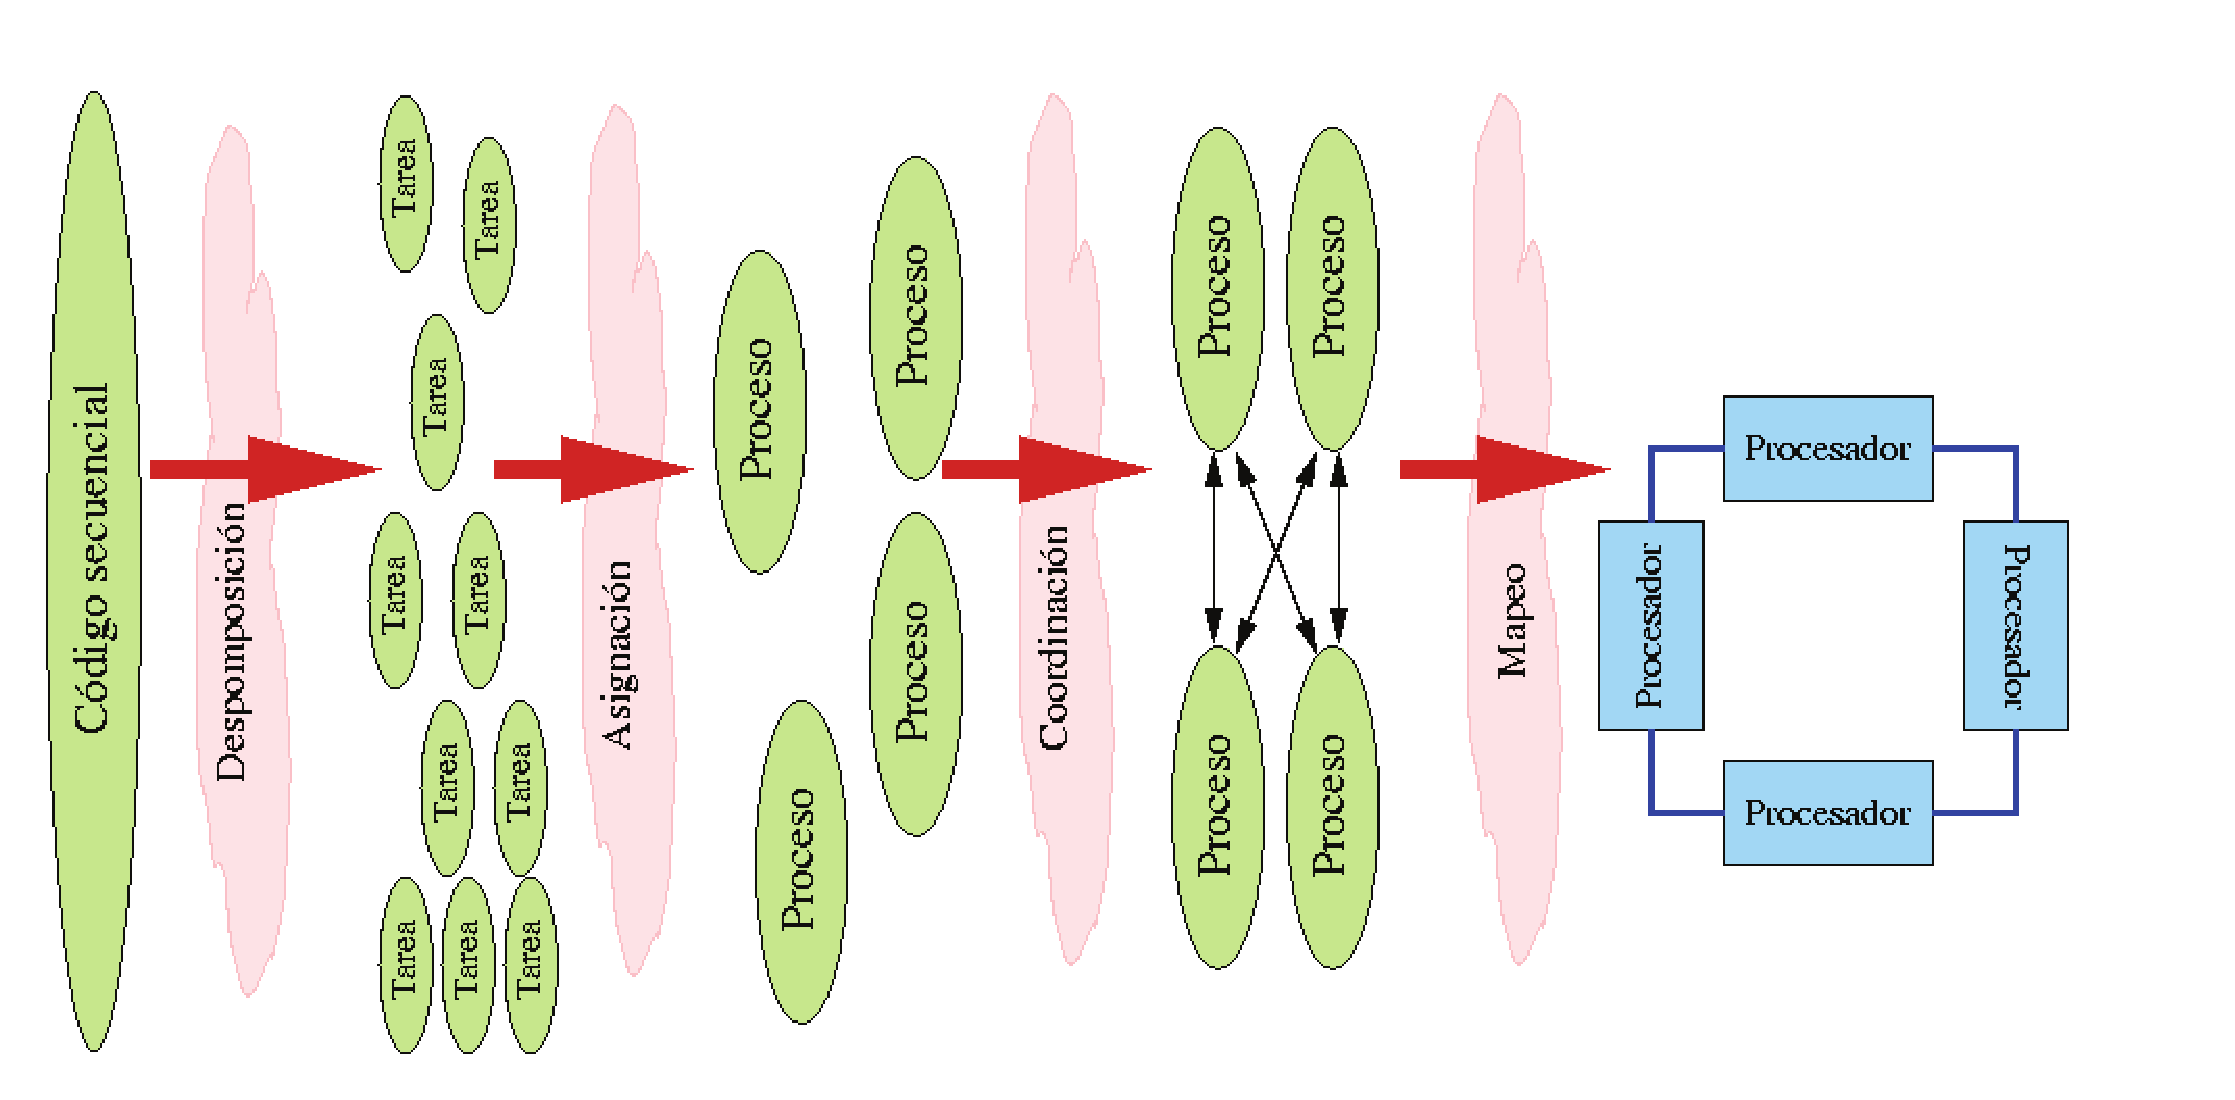
\includegraphics[width=15cm]{figuras/figura01.eps}}
\caption{Esta é a figura de tal e cal.}
\label{enlace1}
\end{figure}

\begin{table}
\begin{center}
\begin{tabular}{|l||r|c|} \hline
Izquierda & Derecha & Centrado  \\ \hline\hline
ll & r & cccc \\ \hline
llll & rrr & c \\ \hline
\end{tabular}
\caption{Esta é a táboa de tal e cal.}
\label{enlace2}
\end{center}
\end{table}

\section{Exemplos de referencias á bibliografía}
Este é un exemplo de referencia a un documento descargado da web \cite{cuda}. E este é un exemplo de referencia a unha páxina da wikipedia \cite{cdma}. Agora un libro \cite{gonzalez} e agora unha referencia a un artigo dunha revista \cite{patricia}. Tamén se poden pór varias referencias á vez \cite{cuda,gonzalez}.

\section{Exemplos de enumeracións}

Con puntos:

\begin{itemize}
\item Un.
\item Dous.
\item Tres.
\end{itemize}

Con números:

\begin{enumerate}
\item Catro.
\item Cinco.
\item Seis.
\end{enumerate}

Exemplo de texto verbatim:

\begin{verbatim}
O texto        verbatim 
     se visualiza tal
            como se escribe
\end{verbatim}

Exemplo de código C:

\lstset{language=C}

\begin{lstlisting}
#include <math.h>
main()
{  int i, j, a[10];
   for(i=0;i<=10;i++) a[i]=i; // comentario 1
   if(a[1]==0) j=1; /* comentario 2 */
   else j=2;
}
\end{lstlisting}

Exemplo de código Java:

\lstset{language=java}

\begin{lstlisting}
class HelloWorldApp {
    public static void main(String[] args) {
        System.out.println("Hello World!"); // Display the string.
    }
}
\end{lstlisting}



%
% Engadir os capitulos que fagan falta
%
\cleardoublepage
\chapter{Conclusións e posibles ampliacións}

Conclusións e posibles ampliacións


% Aquí empezan os apéndices
\appendix
\cleardoublepage
\chapter{Manual técnico: API de Demiurgo}
\renewcommand\theadfont{\bfseries}
\renewcommand\cellalign{ll}

Os servizos web tipo REST son o xeito que teñen o DemiurgoWeb e outras posibles
interfaces de comunicarse co Demiurgo. A comunicación realízase mediante
conexións HTTP mediante GET ou POST, dependendo do método, que envían e reciben
obxectos JSON.
\par
Neste manual especificaranse os distintos tipos de datos e os métodos
dispoñibles para que calquera desenvolvedor poida implementar novas interfaces.

\section{Tipos de datos}
Os tipos de datos definen a estrutura JSON dos datos que se envían e reciben a
través dos métodos. Para simplificar a lectura clasificaremos estes tipos en
dúas categorías: tipos básicos e tipos complexos.

\subsection{Tipos básicos}
Os tipos básicos son os obxectos JSON que fan referencia a elementos
fundamentais do sistema, tales como obxectos, escenarios ou usuarios. Na maioría
dos casos estes obxectos correspóndense en gran medida co modelo de datos
empregado internamente polo Demiurgo.

\subsubsection{Action}
Obxecto que se corresponde cunha acción determinada. Contén toda a información
relativa á acción, polo que non se envía nunca aos xogadores, só aos DX.
\begin{tabular} { | l | l | l | l | }
\hline
\thead{Campo} & \thead{Tipo} & \thead{Opcional} & \thead{Descrición} \\
\hline
id & Enteiro & non & Identificador único da acción. \\
\hline
narration & Texto & non & Narración textual da acción. \\
\hline
room & Texto & non & \makecell{Nome do escenario no que se \\ desenvolve a
acción.}
\\
\hline
witnesses & Lista: Witness & non & \makecell{Lista das testemuñas da
acción; \\ é dicir, os usuarios que teñen \\ acceso a esta acción.} \\
\hline
date & Texto & non & Data na que se creou a acción. \\
\hline
published & Booleano & non & \makecell{Estado da acción. Verdadeiro \\ no caso
de tratarse dunha \\ acción publicada; falso se aínda \\ non foi publicada. As
accións \\ só se publican cando se redacta \\ a súa correspondente narración.}
\\
\hline
\end{tabular}

\subsubsection{Class}
Correspóndese cunha clase do sistema de xogo, a partir da cal poden herdar
os obxectos.

\begin{tabular} { | l | l | l | l | }
\hline
\thead{Campo} & \thead{Tipo} & \thead{Opcional} & \thead{Descrición} \\
\hline
classname & Texto & non & Nome da clase. \\
\hline
parent & Class & si & Clase pai da que herda. \\
\hline
fields & Lista: Variable & non & Lista de campos da clase. \\
\hline
methods & Lista: Method & non & Lista de métodos. \\
\hline
code & Texto & non & Código COE da clase. \\
\hline
\end{tabular}

\subsubsection{Inventory}
Correspóndese cun inventario dun obxecto. Esta clase non fai referencia ao campo
de tipo \textit{inventario} do obxecto, senón ao inventario en si e os obxectos
que contén.

\begin{tabular} { | l | l | l | l | }
\hline
\thead{Campo} & \thead{Tipo} & \thead{Opcional} & \thead{Descrición} \\
\hline
name & Texto & non & \makecell{Nome do inventario, que se \\ corresponde co nome
do campo.}
\\
\hline
objects & Lista: Object & non & \makecell{Lista de obxectos que contén o \\
inventario.}
\\
\hline
\end{tabular}

\subsubsection{Method}
Método asociado a unha clase. Contén o nome e o nome dos argumentos.

\begin{tabular} { | l | l | l | l | }
\hline
\thead{Campo} & \thead{Tipo} & \thead{Opcional} & \thead{Descrición} \\
\hline
name & Texto & non & Nome do método. \\
\hline
args & Lista: Texto & non & \makecell{Lista de argumentos de entrada \\ do
método.}
\\
\hline
returnArg & Texto & non & Nome do argumento de saída. \\
\hline
\end{tabular}

\subsubsection{Object}
Contén a información dun obxecto do mundo de xogo.

\begin{tabular} { | l | l | l | l | }
\hline
\thead{Campo} & \thead{Tipo} & \thead{Opcional} & \thead{Descrición} \\
\hline
id & Enteiro & non & \makecell{Identificador único do \\ obxecto.} \\
\hline
classname & Texto & non & Nome da clase do obxecto. \\
\hline
locationId & Enteiro & non & Identificador da localización. \\
\hline
fields & Lista: Variable & non & Lista de campos do obxecto. \\
\hline
methods & Lista: Method & non & Lista de métodos da clase. \\
\hline
inventories & Lista: Inventory & non & \makecell{Lista de inventarios do \\
obxecto.} \\
\hline
\end{tabular}

\subsubsection{Room}
Correspóndese cun escenario do mundo de xogo. Contén as variables do escenario e
tamén a lista de obxectos que se atopan nel.

\begin{tabular} { | l | l | l | l | }
\hline
\thead{Campo} & \thead{Tipo} & \thead{Opcional} & \thead{Descrición} \\
\hline
id & Enteiro & non & \makecell{Identificador único da \\ localización.} \\
\hline
longPath & Texto & non & Nome completo do escenario. \\
\hline
variables & Lista: Variable & non & \makecell{Lista de variables de \\
escenario.}
\\
\hline
objects & Lista: Object & non & \makecell{Lista de obxectos contidos no \\
escenario.}
\\
\hline
users & Lista: User & non & \makecell{Lista de usuarios con \\ personaxes no
escenario.}
\\
\hline
prenarration & Texto & si & \makecell{Prenarración do escenario, \\ xerada
mediante os \\ comandos ``echo'' \\ invocados mediante o \\ código.}
\\
\hline
\end{tabular}

\subsubsection{Status Inventory}
Obxecto especial. Fai referencia a un inventario tal e como é percibido por un
usuario. Non contén todos os datos que contén un obxecto Inventory.

\begin{tabular} { | l | l | l | l | }
\hline
\thead{Campo} & \thead{Tipo} & \thead{Opcional} & \thead{Descrición} \\
\hline
name & Texto & non & Nome do inventario. \\
\hline
objects & Lista: Object & non &  Lista de obxectos no inventario.\\
\hline
\end{tabular}

\subsubsection{Status Object}
Obxecto especial. Fai referencia a un obxecto do mundo de xogo tal e como é
percibido por un usuario. Non contén todos os datos que contén un obxecto
Object.

\begin{tabular} { | l | l | l | l | }
\hline
\thead{Campo} & \thead{Tipo} & \thead{Opcional} & \thead{Descrición} \\
\hline
name & Texto & non & \makecell{Nome do obxecto, definido \\ polo campo
``v\_name''.
No \\ caso de non ter tal campo, \\ o nome será o nome da clase.}
\\
\hline
description & Texto & si & \makecell{Descrición do obxecto, definida \\ polo
campo ``v\_description''.}
\\
\hline
imgUrl & Texto & si & \makecell{Imaxe do obxecto, definida \\ polo campo
``v\_imgurl''.} \\
\hline
fields & Lista: Variable & non & \makecell{Lista de campos do obxecto \\
visibles para o usuario.}
\\
\hline
inventories & \makecell{Lista: Status \\ Inventory} & non & \makecell{Lista de
inventarios do obxecto \\
visibles para o usuario.} \\
\hline
\end{tabular}

\subsubsection{User}
Contén os datos asociados a un usuario.

\begin{tabular} { | l | l | l | l | }
\hline
\thead{Campo} & \thead{Tipo} & \thead{Opcional} & \thead{Descrición} \\
\hline
name & Texto & non & Nome do usuario. \\
obj & Object & si & Personaxe do usuario, en caso de telo. \\
decision & Texto & si & \makecell{Decisión do usuario, en caso de ter \\ escrito
unha.}
\\
role & Texto & non & \makecell{Rol do usuario. Dous roles \\ dispoñibles:
``gm'' e ``user''.}
\\
\hline
\end{tabular}

\subsubsection{Variable}
Este obxecto contén información sobre unha variable de escenario, un campo dun
obxecto ou un campo definido nunha clase. Contén o nome da variable, o seu valor
en forma de cadea de texto, e o seu tipo.

\begin{tabular} { | l | l | l | l | }
\hline
\thead{Campo} & \thead{Tipo} & \thead{Opcional} & \thead{Descrición} \\
\hline
name & Texto & non & Nome da variable ou campo. \\
\hline
value & Texto & non & Valor textual da variable ou campo. \\
\hline
type & Texto & non & \makecell{Tipo da variable ou campo. Os tipos \\
dispoñibles pódense atopar no manual \\ da linguaxe COE
(apéndice \ref{ch:manual}).}
\\
\hline
\end{tabular}


\subsubsection{Witness}
Obxecto auxiliar que serve para identificar ás testemuñas dunha acción. As
testemuñas son os usuarios involucrados na acción, é dicir, que teñen personaxes
no escenario no momento de suceder a acción.

\begin{tabular} { | l | l | l | l | }
\hline
\thead{Campo} & \thead{Tipo} & \thead{Opcional} & \thead{Descrición} \\
\hline
user & Texto & non & Nome do usuario. \\
\hline
decision & Texto & si & Decisión do usuario en caso de tela. \\
\hline
\end{tabular}


\subsection{Tipos complexos}
Os tipos complexos non se corresponden con elementos do modelo de datos; no seu
lugar, serven para agrupar diferentes tipos básicos. A maioría de métodos que
devolven un obxecto JSON como resposta devolven un tipo complexo.

\subsubsection{AllClasses Response}
Resposta ao método \textit{allclasses}. Contén unha árbore de clases
estruturadas segundo a herdanza.

\begin{tabular} { | l | l | l | l | }
\hline
\thead{Campo} & \thead{Tipo} & \thead{Opcional} & \thead{Descrición} \\
\hline
classes & ClassTree & non & \makecell{Clase raíz ``object" que contén ao
\\ resto.}
\\
\hline
\end{tabular}

\subsubsection{AllRoomPaths Response}
Resposta ao método \textit{roompaths}. Contén unha lista con todos os
nomes de escenarios.

\begin{tabular} { | l | l | l | l | }
\hline
\thead{Campo} & \thead{Tipo} & \thead{Opcional} & \thead{Descrición} \\
\hline
status & \makecell{Status \\ Response} & non & Resposta co estado da operación.
\\
\hline
paths & Lista: Texto & non & Lista de nomes de escenario. \\
\hline
\end{tabular}

\subsubsection{ChangePassword Request}
Datos para a petición de cambio de contrasinal mediante o método
\textit{changepasswd}.

\begin{tabular} { | l | l | l | l | }
\hline
\thead{Campo} & \thead{Tipo} & \thead{Opcional} & \thead{Descrición} \\
\hline
username & Texto & non & Nome do usuario. \\
\hline
oldPassword & Texto & non & Contrasinal anterior. \\
\hline
newPassword & Texto & non & Contrasinal novo. \\
\hline
\end{tabular}

\subsubsection{CheckRoom Response}
Resposta ao método \textit{checkroom}. Contén un obxecto de tipo \textit{Room}
e, no caso de haber algunha acción sen resolver, o obxecto \textit{Action}
correspondente.

\begin{tabular} { | l | l | l | l | }
\hline
\thead{Campo} & \thead{Tipo} & \thead{Opcional} & \thead{Descrición} \\
\hline
status & \makecell{Status \\ Response} & non & \makecell{Resposta co estado da
\\ operación.}
\\
\hline
room & Room & non & Escenario solicitado. \\
\hline
unpublishedAction & Action & si & \makecell{Acción sen resolver, no caso \\ de
que haxa unha.}
\\
\hline
\end{tabular}

\subsubsection{ClassTree}
Obxecto intermedio empregado para facer árbores de clases baseándose na súa
herdanza.

\begin{tabular} { | l | l | l | l | }
\hline
\thead{Campo} & \thead{Tipo} & \thead{Opcional} & \thead{Descrición} \\
\hline
className & Texto & non & \makecell{Nome da clase que se \\ corresponde con este
nodo.}
\\
\hline
children & Lista: ClassTree & si & \makecell{Lista de clases fillas.}
\\
\hline
\end{tabular}

\subsubsection{CreateClass Request}
Datos da petición de creación dunha clase do xogo.

\begin{tabular} { | l | l | l | l | }
\hline
\thead{Campo} & \thead{Tipo} & \thead{Opcional} & \thead{Descrición} \\
\hline
name & Texto & non & Nome da clase. \\
\hline
code & Texto & non & Código COE de definición da clase. \\
\hline
\end{tabular}

\subsubsection{CreateClass Response}
Resposta á petición de creación dunha clase do xogo.

\begin{tabular} { | l | l | l | l | }
\hline
\thead{Campo} & \thead{Tipo} & \thead{Opcional} & \thead{Descrición} \\
\hline
status & \makecell{Status \\ Response} & non & Resposta co estado da operación.
\\
\hline
createdClass & Class & non & Devolve a clase creada. \\
\hline
\end{tabular}

\subsubsection{CreateRoom Request}
Datos da petición de creación dun escenario. É un obxecto moi sinxelo que só
contén o nome do escenario.

\begin{tabular} { | l | l | l | l | }
\hline
\thead{Campo} & \thead{Tipo} & \thead{Opcional} & \thead{Descrición} \\
\hline
path & Texto & non & \makecell{Nome completo do escenario.} \\
\hline

\hline
\end{tabular}

\subsubsection{DeleteVariable Request}
Datos da petición de borrado dunha variable de escenario.

\begin{tabular} { | l | l | l | l | }
\hline
\thead{Campo} & \thead{Tipo} & \thead{Opcional} & \thead{Descrición} \\
\hline
path & Texto & non & \makecell{Nome do escenario que contén a variable.}
\\
\hline
varName & Texto & non & \makecell{Nome da variable.}
\\
\hline
\end{tabular}

\subsubsection{DeleteVariable Response}
Resposta á petición de borrado dunha variable de escenario.

\begin{tabular} { | l | l | l | l | }
\hline
\thead{Campo} & \thead{Tipo} & \thead{Opcional} & \thead{Descrición} \\
\hline
status & \makecell{Status \\ Response} & non & Resposta co estado da operación.
\\
\hline
\end{tabular}

\subsubsection{DestroyClass Request}
Datos da petición de destrución dunha clase do xogo.

\begin{tabular} { | l | l | l | l | }
\hline
\thead{Campo} & \thead{Tipo} & \thead{Opcional} & \thead{Descrición} \\
\hline
className & Texto & non & \makecell{Nome da clase a borrar.}
\\
\hline
\end{tabular}

\subsubsection{DestroyClass Response}
Resposta á petición de destrución dunha clase do xogo.

\begin{tabular} { | l | l | l | l | }
\hline
\thead{Campo} & \thead{Tipo} & \thead{Opcional} & \thead{Descrición} \\
\hline
status & \makecell{Status \\ Response} & non & Resposta co estado da operación.
\\
\hline
\end{tabular}

\subsubsection{DestroyObject Request}
Datos da petición de destrución dun obxecto do mundo.

\begin{tabular} { | l | l | l | l | }
\hline
\thead{Campo} & \thead{Tipo} & \thead{Opcional} & \thead{Descrición} \\
\hline
objId & Enteiro & non & \makecell{Identificador do obxecto a \\ borrar.}
\\
\hline
destroyContents & Booleano & non & \makecell{Se é verdadeiro, destruiranse \\
todos os obxectos contidos \\ nos inventarios do obxecto. \\ Se é falso, serán
desprazados \\ ao escenario no que se atopa \\  o obxecto en cuestión.}
\\
\hline
\end{tabular}

\subsubsection{DestroyObject Response}
Resposta á petición de destrución dun obxecto do mundo.

\begin{tabular} { | l | l | l | l | }
\hline
\thead{Campo} & \thead{Tipo} & \thead{Opcional} & \thead{Descrición} \\
\hline
status & \makecell{Status \\ Response} & non & Resposta co estado da operación.
\\
\hline
\end{tabular}

\subsubsection{DestroyRoom Request}
Datos da petición de destrución dun escenario.

\begin{tabular} { | l | l | l | l | }
\hline
\thead{Campo} & \thead{Tipo} & \thead{Opcional} & \thead{Descrición} \\
\hline
path & Texto & non & \makecell{Nome completo do escenario.}
\\
\hline
\end{tabular}

\subsubsection{DestroyRoom Response}
Resposta á petición de destrución dun escenario.

\begin{tabular} { | l | l | l | l | }
\hline
\thead{Campo} & \thead{Tipo} & \thead{Opcional} & \thead{Descrición} \\
\hline
status & \makecell{Status \\ Response} & non & Resposta co estado da operación.
\\
\hline
\end{tabular}

\subsubsection{ExecuteCode Request}
Datos da petición de execución de código.

\begin{tabular} { | l | l | l | l | }
\hline
\thead{Campo} & \thead{Tipo} & \thead{Opcional} & \thead{Descrición} \\
\hline
path & Texto & non & \makecell{Nome do escenario no que se \\ executará o
código.}
\\
\hline
code & Texto & non & \makecell{Código COE a executar.}
\\
\hline
createAction & Booleano & non & \makecell{Se é verdadeiro, crearase unha \\ nova
acción sen publicar e \\\ solicitarase unha narración ao \\ DX. Se é falso,
non se crearán \\ accións.}
\\
\hline
\end{tabular}

\subsubsection{ExecuteCode Response}
Resposta á petición de execución de código.

\begin{tabular} { | l | l | l | l | }
\hline
\thead{Campo} & \thead{Tipo} & \thead{Opcional} & \thead{Descrición} \\
\hline
status & \makecell{Status \\ Response} & non & Resposta co estado da operación.
\\
\hline
action & Action & si & Acción creada no caso de existir unha. \\
\hline
\end{tabular}

\subsubsection{GetPendingRooms Response}
Resposta á petición de escenarios activos.

\begin{tabular} { | l | l | l | l | }
\hline
\thead{Campo} & \thead{Tipo} & \thead{Opcional} & \thead{Descrición} \\
\hline
status & \makecell{Status \\ Response} & non & \makecell{Resposta co estado da
\\ operación.}
\\
\hline
pendingRooms & \makecell{Lista: Pending \\ Room} & non & Lista de escenarios
activos.
\\
\hline
numUsers & Enteiro & non & \makecell{Número de usuarios en \\ xogo.} \\
\hline
noObjUsers & Lista: User & non & \makecell{Lista de usuarios sen un \\ personaxe
asignado.}
\\
\hline
\end{tabular}

\subsubsection{Login Request}
Datos da petición de \textit{login}.

\begin{tabular} { | l | l | l | l | }
\hline
\thead{Campo} & \thead{Tipo} & \thead{Opcional} & \thead{Descrición} \\
\hline
name & Texto & non & \makecell{Nome de usuario.}
\\
\hline
password & Texto & non & \makecell{Contrasinal do usuario.}
\\
\hline
world & Texto & non & Nome do mundo. \\
\hline
\end{tabular}

\subsubsection{Me Response}
Resposta á petición de datos do usuario.

\begin{tabular} { | l | l | l | l | }
\hline
\thead{Campo} & \thead{Tipo} & \thead{Opcional} & \thead{Descrición} \\
\hline
status & \makecell{Status \\ Response} & non & Resposta co estado da operación.
\\
\hline
user & User & non & Datos do usuario. \\
\hline
obj & \makecell{Status \\ Object} & si & Personaxe do usuario. \\
\hline
world & Texto & non & Mundo ao que pertence o usuario. \\
\hline
\end{tabular}

\subsubsection{NarrateAction Request}
Datos da petición de narración dunha acción.

\begin{tabular} { | l | l | l | l | }
\hline
\thead{Campo} & \thead{Tipo} & \thead{Opcional} & \thead{Descrición} \\
\hline
id & Enteiro & non & \makecell{Identificador da acción.}
\\
\hline
narration & Texto & non & \makecell{Narración da acción.}
\\
\hline
\end{tabular}

\subsubsection{NarrateAction Response}
Resposta á petición de narración dunha acción.

\begin{tabular} { | l | l | l | l | }
\hline
\thead{Campo} & \thead{Tipo} & \thead{Opcional} & \thead{Descrición} \\
\hline
status & \makecell{Status \\ Response} & non & Resposta co estado da operación.
\\
\hline
action & Action & non & Acción modificada. \\
\hline
\end{tabular}

\subsubsection{PastActions Response}
Resposta á petición de accións pasadas do xogador.

\begin{tabular} { | l | l | l | l | }
\hline
\thead{Campo} & \thead{Tipo} & \thead{Opcional} & \thead{Descrición} \\
\hline
status & \makecell{Status \\ Response} & non & \makecell{Resposta co estado da
\\ operación.}
\\
\hline
totalActions & Enteiro & non & \makecell{Total de accións visibles \\ para o
xogador.}
\\
\hline
actions & Lista: Texto & non & \makecell{Lista co texto das accións \\
solicitadas.}
\\
\hline
\end{tabular}

\subsubsection{Pending Room}
Obxecto que contén os datos relativos a un escenario activo.

\begin{tabular} { | l | l | l | l | }
\hline
\thead{Campo} & \thead{Tipo} & \thead{Opcional} & \thead{Descrición} \\
\hline
path & Texto & non & Nome completo do escenario. \\
\hline
numObjects & Enteiro & non & \makecell{Total de obxectos no \\ escenario.} \\
\hline
numUsers & Enteiro & non & \makecell{Total de xogadores no \\ escenario.} \\
\hline
decidingUsers & Lista: Texto & non & \makecell{Nome dos xogadores que \\
mandaron decisións.}
\\
\hline
\end{tabular}

\subsubsection{RegisterUser Request}
Datos da petición de rexistro dun usuario.

\begin{tabular} { | l | l | l | l | }
\hline
\thead{Campo} & \thead{Tipo} & \thead{Opcional} & \thead{Descrición} \\
\hline
world & Texto & non & \makecell{Nome do mundo onde se rexistra o \\ usuario.}
\\
\hline
username & Texto & non & \makecell{Nome do usuario.}
\\
\hline
password & Texto & non & Contrasinal do usuario. \\
\hline
mail & Texto & non & \makecell{Enderezo de correo electrónico do \\ usuario.} \\
\hline
\end{tabular}

\subsubsection{RegisterUser Response}
Resposta á petición de rexistro dun usuario.

\begin{tabular} { | l | l | l | l | }
\hline
\thead{Campo} & \thead{Tipo} & \thead{Opcional} & \thead{Descrición} \\
\hline
status & \makecell{Status \\ Response} & non & Resposta co estado da operación.
\\
\hline
active & Booleano & non & \makecell{Se é verdadeiro, a conta está activa e \\ o
xogador pode comezar a xogar \\ inmediatamente.}
\\
\hline
\end{tabular}

\subsubsection{Response Status}
Obxecto auxiliar que acompaña ás respostas indicando se a operación se executou
correctamente ou houbo algún problema.

\begin{tabular} { | l | l | l | l | }
\hline
\thead{Campo} & \thead{Tipo} & \thead{Opcional} & \thead{Descrición} \\
\hline
ok & Booleano & non & \makecell{Se é verdadeiro, a operación \\ executouse
correctamente. Se é \\ falso, houbo algún problema.}
\\
\hline
description & Texto & si & \makecell{No caso de haber algún problema, \\ devolve
unha descrición do mesmo.}
\\
\hline
\end{tabular}

\subsubsection{RoomHistory Response}
Resposta á petición de historial dun escenario.

\begin{tabular} { | l | l | l | l | }
\hline
\thead{Campo} & \thead{Tipo} & \thead{Opcional} & \thead{Descrición} \\
\hline
status & \makecell{Status \\ Response} & non & \makecell{Resposta co estado da
\\ operación.}
\\
\hline
actions & Lista: Action & non & Lista coas accións devoltas. \\
\hline
totalActions & Enteiro & non & Total de accións do escenario. \\
\hline
\end{tabular}

\subsubsection{SubmitDecision Request}
Datos da petición de envío dunha decisión.

\begin{tabular} { | l | l | l | l | }
\hline
\thead{Campo} & \thead{Tipo} & \thead{Opcional} & \thead{Descrición} \\
\hline
decision & Texto & non & \makecell{Texto da decisión do usuario.}
\\
\hline
\end{tabular}

\subsubsection{WorldList Response}
Resposta á petición da lista de mundos.

\begin{tabular} { | l | l | l | l | }
\hline
\thead{Campo} & \thead{Tipo} & \thead{Opcional} & \thead{Descrición} \\
\hline
worlds & Lista: Texto & non & \makecell{Lista cos nomes dos mundos \\
dispoñibles.}
\\
\hline
\end{tabular}


\section{Métodos dispoñibles}
Nesta sección especificaremos os métodos que ofrece a API. Por cada método
indicarase, ademais dunha breve descrición: se é unha petición HTTP por método
GET ou POST, o obxecto JSON que devolve, e os parámetros que require. Por cada
parámetro especificarase o nome no caso de ir por GET; nos métodos POST deberán
ir no corpo da petición.

\subsection{Métodos de autentificación}
Estes métodos chámanse sen estar identificado polo sistema. Empréganse por tanto
para xestionar a autentificación e rexistro de usuarios.

\subsubsection{login}
Método POST. Identifica o usuario co seu nome e contrasinal no mundo
especificado. Devolve unha cadea de texto coñecida como \textit{token}, que
deberá ser especificada nos distintos métodos que requiran autentificación. O
token inclúese dentro da cabeceira HTTP no campo \textit{Authorization} da
seguinte forma:
\begin{lstlisting}
Authorization: Bearer <token>
\end{lstlisting}

\begin{tabular} {| l | l | l | l |}
\hline
\thead{Parámetro} & \thead{Tipo} & \thead{Opcional} & \thead{Descrición} \\
\hline
(POST) & Login Request & non & Datos de usuario. \\
\hline
\end{tabular}

\subsubsection{register}
Método POST. Rexistra un novo usuario cos datos proporcionados. Devolve un
obxecto \textit{RegisterUser Response}.

\begin{tabular} {| l | l | l | l |}
\hline
\thead{Parámetro} & \thead{Tipo} & \thead{Opcional} & \thead{Descrición} \\
\hline
(POST) & RegisterUser Request & non & Datos de usuario. \\
\hline
\end{tabular}

\subsection{Métodos xenéricos}
Os métodos xenéricos poden ser empregado sen importar o rol do usuario. A súa
función está vinculada principalmente aos propios datos do usuario, e non a
elementos funcionais do xogo.

\subsubsection{changepasswd}
Método POST. Emprégase para cambiar o contrasinal do usuario. Devolve un obxecto
\textit{Response Status}.

\begin{tabular} {| l | l | l | l |}
\hline
\thead{Parámetro} & \thead{Tipo} & \thead{Opcional} & \thead{Descrición} \\
\hline
(POST) & \makecell{ChangePassword \\ Request} & non & \makecell{Contén o
contrasinal vello e \\ o novo.}
\\
\hline
\end{tabular}

\subsubsection{me}
Método GET. Útil para recibir información do usuario e, no caso de tratarse dun
xogador, obter un estado do personaxe. Devolve un obxecto \textit{Me
Response}.

O método \textit{me} non ten parámetros.


\subsection{Métodos para xogadores}
Os xogadores contan só con dous métodos: un para enviar novas decisións, e outro
para ler accións. Isto débese ao feito de que os usuarios nunca perciben
directamente o mundo de xogo, só acceden á información que o DX lles ofrece.

\subsubsection{pastactions}
Método GET. Devolve as narracións das últimas accións. É posible especificar un
rango de accións concreto. As narracións obtidas con este método estarán
filtradas no caso de conter fragmentos ocultos para o xogador. Devolve un
obxecto \textit{PastActions Response}.

\begin{tabular} {| l | l | l | l |}
\hline
\thead{Parámetro} & \thead{Tipo} & \thead{Opcional} & \thead{Descrición} \\
\hline
first & Texto & si & \makecell{Índice da primeira acción que se \\ desexa 
recibir. Debe ser convertible a \\ un número enteiro. Se o valor é \\ negativo,
calcularase a primeira acción \\ restando o valor dende a última acción \\
dispoñible. O valor por defecto é -10.}
\\
\hline
count & Texto & si & \makecell{Número de accións que se queren \\ recibir dende
a primeira. Debe ser \\ convertible  un número enteiro. Por \\ defecto este
valor é 10.}
\\
\hline
\end{tabular}

\subsubsection{submitdecision}
Método POST. Envía unha decisión redactada polo usuario. Non devolve ningún
obxecto.

\begin{tabular} {| l | l | l | l |}
\hline
\thead{Parámetro} & \thead{Tipo} & \thead{Opcional} & \thead{Descrición} \\
\hline
(POST) & \makecell{SubmitDecision \\ Request} & non & \makecell{Contén a
decisión do \\ usuario.}
\\
\hline
\end{tabular}


\subsection{Métodos para o DX}
Os métodos do DX son os que xestionan a partida, ofrecendo ao DX unha canle para
executar código e recibir información do mundo de xogo. Ademais disto, tamén
ofrece métodos útiles para realizar modificacións no mundo directamente.

\subsubsection{action}
Método GET. Emprégase para recibir a información dunha acción concreta. Devolve
un obxecto \textit{Action}.

\begin{tabular} {| l | l | l | l |}
\hline
\thead{Parámetro} & \thead{Tipo} & \thead{Opcional} & \thead{Descrición} \\
\hline
id & Enteiro & non & Identificador único da acción. \\
\hline
\end{tabular}

\subsubsection{allclasses}
Método GET. Emprégase para obter unha árbore de todas as clases no mundo de
xogo. As clases están organizadas segundo a herdanza, comezando pola clase que
fai de raíz: a clase \textit{Object}. As clases que herdan directamente de
\textit{Object} aparecen como fillas deste primeiro nodo, e así sucesivamente.
Devolve un obxecto \textit{AllClasses Response}.

O método \textit{allclasses} non ten parámetros.

\subsubsection{checkroom}
Método GET. Serve para comprobar o estado dun escenario. Ademais do escenario
en si, se existe algunha acción sen publicar, este método serve para chegar a
ela. Devolve un obxecto \textit{CheckRoom Response}.

\begin{tabular} {| l | l | l | l |}
\hline
\thead{Parámetro} & \thead{Tipo} & \thead{Opcional} & \thead{Descrición} \\
\hline
path & Texto & non & Nome completo do escenario. \\
\hline
\end{tabular}

\subsubsection{createclass}
Método POST. Método empregado para crear clases novas. Devolve un obxecto
\textit{CreateClass Response}.

\begin{tabular} {| l | l | l | l |}
\hline
\thead{Parámetro} & \thead{Tipo} & \thead{Opcional} & \thead{Descrición} \\
\hline
(POST) & \makecell{CreateClass \\ Request} & non & Nome e código da clase. \\
\hline
\end{tabular}

\subsubsection{createroom}
Método POST. Método empregado para crear novos escenarios. Devolve un obxecto
\textit{Room} correspondente ao escenario creado.

\begin{tabular} {| l | l | l | l |}
\hline
\thead{Parámetro} & \thead{Tipo} & \thead{Opcional} & \thead{Descrición} \\
\hline
(POST) & \makecell{CreateRoom \\ Request} & non & Especifica o escenario a
borrar.
\\
\hline
\end{tabular}

\subsubsection{delvar}
Método POST. Indica unha variable de escenario para que sexa borrada. Devolve un
obxecto \textit{DeleteVariable Response}.

\begin{tabular} {| l | l | l | l |}
\hline
\thead{Parámetro} & \thead{Tipo} & \thead{Opcional} & \thead{Descrición} \\
\hline
(POST) & \makecell{DeleteVariable \\ Request} & non & Especifica a variable a
borrar.
\\
\hline
\end{tabular}

\subsubsection{destroyclass}
Método POST. Destrúe unha clase do xogo. Devolve un obxecto \textit{DestroyClass
Response}.

\begin{tabular} {| l | l | l | l |}
\hline
\thead{Parámetro} & \thead{Tipo} & \thead{Opcional} & \thead{Descrición} \\
\hline
(POST) & \makecell{DestroyClass \\ Request} & non & Especifica a clase a borrar.
\\
\hline
\end{tabular}

\subsubsection{destroyobj}
Método POST. Destrúe un obxecto do mundo de xogo. Devolve un obxecto
\textit{DestroyObject Response}.

\begin{tabular} {| l | l | l | l |}
\hline
\thead{Parámetro} & \thead{Tipo} & \thead{Opcional} & \thead{Descrición} \\
\hline
(POST) & \makecell{DestroyObject \\ Request} & non & Especifica o obxecto a
borrar.
\\
\hline
\end{tabular}

\subsubsection{destroyroom}
Método POST. Destrúe un escenario. Devolve un obxecto \textit{DestroyRoom
Response}.

\begin{tabular} {| l | l | l | l |}
\hline
\thead{Parámetro} & \thead{Tipo} & \thead{Opcional} & \thead{Descrición} \\
\hline
(POST) & \makecell{DestroyRoom \\ Request} & non & \makecell{Especifica o
escenario a \\ borrar.}
\\
\hline
\end{tabular}

\subsubsection{executecode}
Método POST. Executa código COE nun escenario, podendo xerarse unha acción ou
non segundo se especifique. Devolve un obxecto \textit{ExecuteCode Response}.

\begin{tabular} {| l | l | l | l |}
\hline
\thead{Parámetro} & \thead{Tipo} & \thead{Opcional} & \thead{Descrición} \\
\hline
(POST) & \makecell{ExecuteCode \\ Request} & non & \makecell{Contén o código e
outros \\ datos adicionais.}
\\
\hline
\end{tabular}

\subsubsection{getclass}
Método GET. Método empregado para obter unha clase do xogo. Devolve un obxecto
\textit{Class}.

\begin{tabular} {| l | l | l | l |}
\hline
\thead{Parámetro} & \thead{Tipo} & \thead{Opcional} & \thead{Descrición} \\
\hline
classname & Texto & non & Nome da clase. \\
\hline
\end{tabular}

\subsubsection{history}
Método GET. Permite acceder ao historial dun escenario. Ten un funcionamento
semellante ao método \textit{pastactions}. Devolve un obxecto
\textit{RoomHistory Response}.

\begin{tabular} {| l | l | l | l |}
\hline
\thead{Parámetro} & \thead{Tipo} & \thead{Opcional} & \thead{Descrición} \\
\hline
path & Texto & non & Nome completo do escenario. \\
\hline
first & Texto & si & \makecell{Índice da primeira acción que se \\ desexa 
recibir. Debe ser convertible a \\ un número enteiro. Se o valor é \\ negativo,
calcularase a primeira acción \\ restando o valor dende a última acción \\
dispoñible. O valor por defecto é -10.}
\\
\hline
count & Texto & si & \makecell{Número de accións que se queren \\ recibir dende
a primeira. Debe ser \\ convertible  un número enteiro. Por \\ defecto este
valor é 10.} \\
\hline
\end{tabular}

\subsubsection{modifyclass}
Método POST. Serve para modificar unha clase xa existente. Devolve un obxecto
\textit{CreateClass Response}, e ten un funcionamento semellante ao método
\textit{createclass}.

\begin{tabular} {| l | l | l | l |}
\hline
\thead{Parámetro} & \thead{Tipo} & \thead{Opcional} & \thead{Descrición} \\
\hline
(POST) & \makecell{CreateClass \\ Request} & non & \makecell{Contén o novo
código COE da \\ clase.}
\\
\hline
\end{tabular}

\subsubsection{narrateaction}
Método POST. Engade a narración a unha acción concreta. No caso de xa contar
cunha narración, sobreescríbea. Devolve un obxecto \textit{NarrateAction
Response}.

\begin{tabular} {| l | l | l | l |}
\hline
\thead{Parámetro} & \thead{Tipo} & \thead{Opcional} & \thead{Descrición} \\
\hline
(POST) & \makecell{NarrateAction \\ Request} & non & \makecell{Contén a
narración da acción.}
\\
\hline
\end{tabular}

\subsubsection{pendingrooms}
Método GET. Método empregado para obter infomación sobre os escenarios activos
e o estado dos xogadores. Devolve un obxecto \textit{PendingRooms Response}.

O método \textit{pendingrooms} non ten parámetros.

\subsubsection{roompaths}
Método GET. Ofrece unha lista de nomes de escenarios no mundo actual. Devolve
un obxecto \textit{AllRoomPaths Response}.

O método \textit{roompaths} non ten parámetros.
\cleardoublepage
\chapter{Manual de usuario}
\label{ch:manual}

\section{Introdución}
A linguaxe COE (acrónimo de Código de Obxectos e Escenarios) é a linguaxe
empregada nas partidas no Demiurgo, o software de xestión de
partidas de rol asíncronas. O director de xogo ({\it DX}) pode escribir código
en COE para definir clases no mundo de xogo, e para realizar accións nos escenarios nas que
os distintos obxectos interactúan entre si.
\par
A finalidade deste manual é definir esta linguaxe e ensinar a darlle uso para
poder empregar todas as funcionalidades do Demiurgo sen dificultade, ofrecendo
para isto definicións formais, explicacións e exemplos en cada apartado. Grazas
a este sistema, o DX pode manter un mundo loxicamente coherente que lle faga de
soporte á hora de levar as partidas, evitando así erros e automatizando en gran
medida o apartado técnico das mesmas.




\section{Escenarios, clases e obxectos}
Un mundo de xogo de Demiurgo está composto por obxectos, cada un dos cales
segue a definición dunha clase e atópase dentro dun escenario. A medida que
a partida avanza, os distintos obxectos créanse, modifícanse, móvense dun
escenario a outro e interactúan entre eles.
\subsection{Exemplo dunha situación}
Expresaremos unha situación normal do xogo mediante este exemplo:
\par
{\it A situación transcorre na taberna da capital do reino. Tres ananos están
nun recuncho discutindo entre eles acaloradamente. Detrás da barra pódese ver ao
taberneiro, un home corpulento que se distrae limpando un vaso. Detrás da barra
ten un mosquetón agochado por se as cousas se poñen feas, e por se acaso non
lle quita ollo aos ananos.}
\par
En base a esta descrición da situación, o director de xogo pode definir
internamente o seguinte:
\begin{itemize}
  \item Un escenario que se corresponde coa {\bf taberna}. O escenario debería
  ter un nome recoñecible para o director de xogo, como por exemplo {\it
  /reino/capital/taberna}, máis iso explicarase máis en detalle
  en \ref{subsec:nome-escenarios}.
  \item Como mínimo {\bf 5 obxectos}: \begin{itemize}
    \item Tres obxectos que representen aos {\bf ananos}. Xa que son tres
    obxectos moi semellantes, o normal é que pertenzan á mesma clase; por
    exemplo, unha clase chamada {\it Anano}. Máis isto non é unha norma,
    dependerá de como o director de xogo teña definido o mundo.
    \item Un obxecto que represente ao {\bf taberneiro}. Pode pertencer a unha
    clase diferenciada da dos ananos (como {\it Humano}); non obstante, ben poden
    pertencer tanto o taberneiro como os ananos a unha mesma clase {\it
    Intelixente} ou {\it Criatura}, por exemplo.
    \item Un obxecto que faga referencia á {\bf barra}, xa que o {\bf mosquetón}
    que contén pode resultar relevante no futuro. Por tanto, o normal sería  que
    houbese un obxecto que representase á barra (de clase {\it Mobiliario} por
    exemplo), e no seu interior se atopase un inventario que conteña ao obxecto
    mosquetón (de clase {\it Mosquetón}). Explicarase con detalle o concepto dos
    inventarios en \ref{subsec:inventarios}.
  \end{itemize}
\end{itemize}
\par
Esta configuración é un simple exemplo que non ten por que cumprirse ao
100\% nunha partida real, pero da unha idea do concepto. Poñamos agora outro
exemplo: na mesma situación, comezan a suceder cousas.
\par
{\it Parece que a discusión dos ananos chega a un punto crítico. Dous deles
deciden simultaneamente que non poderán resolver as súas diferencias mediante a
diplomacia, polo que deciden sacar os puños e golpearse mutuamente. O
taberneiro, que non lles quitaba ollo, saca o mosquetón como resposta por se
comeza unha escalada de violencia.}
\par
Isto pode suceder por dous motivos: os dous ananos son personaxes
controlados por xogadores e ambos tomaron a mesma decisión (golpear ao outro) ao
mesmo tempo; ou ben son personaxes non xogadores ({\it NPC}, {\it non player
character}) e foi o propio DX o que tomou a decisión por eles (para que outros
xogadores no escenario presenciaran isto, por exemplo).
\par
En calquera caso, o que lle corresponde ao DX é executar o código necesario para
cambiar o estado do mundo. O código a redactar debe facer tres cousas:
\begin{enumerate}
  \item Un dos ananos debe {\bf golpear} ao outro, cos cambios que iso implique
  (por exemplo, reducir o seu campo {\it vida}).
  \item O segundo anano debe {\bf golpear} ao primeiro.
  \item O mosquetón debe deixar de estar no inventario da barra e debe
  {\bf moverse} ao inventario do taberneiro.
\end{enumerate}
\par
Este sería un exemplo de como podería ser este código:
\begin{lstlisting}
anano1.golpear(anano2)
anano2.golpear(anano1)
barra.contidos[0] >> taberneiro.inventario
\end{lstlisting}
\par
Como entendemos este código? Temos unha variable anano1 que fai referencia ao
obxecto {\it Anano} que da o primeiro golpe, unha variable anano2 que fai
referencia ao segundo, unha variable {\it barra}, unha variable {\it
taberneiro}, e un método {\it golpear()} definido para a clase {\it Anano}. Este
código enténdese así:
\begin{enumerate}
  \item O obxecto correspondente á variable anano1 executa o {\bf método}
  {\it golpear()}, collendo o obxecto da variable anano2 como argumento. Este
  método, definido na clase {\it Anano}, reduce a vida do anano seleccionado
  como argumento. Explicarase máis en detalle isto na sección
  \ref{subsec:metodos}.
  \item O mesmo que no anterior, pero ao revés.
  \item O primeiro obxecto ({\it [0]}) dos contidos da barra (''contidos'' é un
  inventario da clase {\it Mobiliario}), que neste caso entendemos que é o
  mosquetón, {\bf móvese} (>>) ao inventario do taberneiro. 
\end{enumerate}

\subsection{Escenarios}
\subsubsection{Definición de escenario}
O mundo de xogo está dividido en escenarios (tamén chamados {\it habitacións}
polo seu homólogo {\it rooms} en inglés). Cada escenario está composto por:
\begin{itemize}
  \item O seu nome, sobre o cal falaremos na subsección
  \ref{subsec:nome-escenarios}.
  \item O conxunto de obxectos que se atopan ''dentro'' do escenario.
  \item As variables do escenario, as cales poden conter datos tales como
  números enteiros ou texto, pero tamén referencias a obxectos ou outros
  escenarios.
\end{itemize}
\par
O escenario forma unha unidade lóxica fundamental no mundo de xogo, e o habitual
é que as accións en cada escenario afecten só aos obxectos do propio escenario
(aínda que pode haber excepcións).

\subsubsection{Nome do escenario}
\label{subsec:nome-escenarios}
O nome de escenario serve para que o DX o identifique rapidamente. Ademais de
ofrecer un nome descritivo, o nome completo permite organizar os escenarios
nunha estrutura xerárquica, cunha lóxica semellante á das rutas de ficheiros nos
sistemas operativos.
\par
Exemplo:
\begin{lstlisting}
/continente/reinohumano/cidadecapital/armeria
/continente/reinohumano/cidadecapital/taberna
/continente/reinohumano/aldeacosteira
\end{lstlisting}
\par
Estes tres escenarios atópanse dentro de /continente/reinohumano, é dicir,
na estrutura lóxica do mundo de xogo están dentro do mesmo reino, o cal forma
parte do continente. A maiores, os dous primeiros están na mesma cidade. Estes
compoñentes normalmente reciben o nome de {\it rexións}, pero poden ter o
significado semántico que o DX de xogo prefira, por exemplo, nunha partida
futurista poderíamos atopar algo como:
\begin{lstlisting}
/planetamarte/coloniahumana/suburbios/casa3/cocinha
/planetamarte/orbita/sateliteflotante/laboratorio
/espazoexterior/zonadeasteroides
\end{lstlisting}
\par
Por último, o DX pode renunciar completamente a usar a xerarquía de escenarios,
aínda que iso pode dificultar o nomeado de escenarios:
\begin{lstlisting}
/chairas_da_capital_humana
/sala_do_gran_mago
\end{lstlisting}
\par
É importante ter en conta que o nome dos escenarios só pode estar composto por
caracteres alfanuméricos e barras baixas, e non pode conter letras que non
formen parte do alfabeto inglés (tales como {\it ñ} ou {\it ç}). O nome completo
sempre debe comezar por /. Por último, o Demiurgo non distingue entre
minúsculas e maiúsculas.
\par
Nota: {\it /} en si mesmo pode ser un escenario, o coñecido como {\it escenario
raíz}, pero non é habitual o seu uso.

\subsubsection{Contido do escenario}
O escenario pode conter obxectos (e de feito é habitual que os conteña). Estes
obxectos á súa vez poden dispoñer de inventarios (ver
subsección \ref{subsec:inventarios}) que conteñan outros obxectos. Mediante a
interface gráfica, o DX pode ver os distintos obxectos do escenario para operar
con eles no código.

\subsubsection{Variables}
O DX pode definir variables no escenario a través do código. Estas variables
están accesibles dende o propio escenario e poden ter todo tipo de utilidades.
Por exemplo, é habitual referenciar os obxectos do escenario en variables para
poder manexalos co código máis facilidade.
\par
Exemplo: Imaxinemos que no escenario temos un obxecto que representa a un
trasno. O obxecto ten un identificador propio ({\it ID}) que é \#1234 (ver
sección \ref{sec:obxectos}).
No momento de querer actuar, se non empregamos variables precisamos referirnos a
el co seu ID:
\begin{lstlisting}
#1234.facerTrasnadas()
if(#1234.famento == true)
  ! "O trasno ten bastante fame"
\end{lstlisting}
\par
En cambio, se temos unha variable cun nome descritivo (por exemplo, {\it
trasno}) podemos codificalo así:
\begin{lstlisting}
trasno.facerTrasnadas()
if(trasno.famento == true)
  ! "O trasno ten bastante fame"
\end{lstlisting}
\par
Outro uso frecuente das variables é gardar datos. Neste exemplo tírase un dado
de 20 caras e móstrase un texto ou outro segundo o resultado:
\begin{lstlisting}
int resultado = d20
if(resultado > 10) {
  ! "A accion tivo exito"
}
if(resultado < 3) {
  ! "A accion foi un fracaso absoluto"
}
\end{lstlisting}



\subsection{Clases}
\label{sec:clases}
As clases son definicións empregadas a modo de modelo para crear obxectos. Todos
os obxectos que teñan a mesma clase terán unha serie de métodos e campos
comúns definidos na propia clase.
\par
Nesta sección explicarase como funcionan as clases e todo o relacionado con
elas. No capítulo \ref{ch:definicion} explícase polo miúdo a sintaxe formal para
crear clases.
\subsubsection{Campos}
Os campos son variables vinculadas aos obxectos, e a súa finalidade é
almacenar datos relacionados con eles. Por exemplo, nun mundo de rol de fantasía
medieval, é habitual atopar nos personaxes campos como forza, axilidade ou
intelixencia. Nun mundo con máquinas de guerra, normalmente atoparemos campos
como a potencia de disparo ou o blindaxe. E tamén podemos atopar campos en
obxectos inanimados, como o peso, o prezo, a cor, etcéra.
\par
Os campos defínense coa clase, e cando é creado un obxecto desa clase,
automaticamente pasa a posuír todos os campos da mesma.
\par
Exemplo:
\begin{lstlisting}
elfo {
  int forza = 1
  int axilidade = 3
  int constitucion = 1
  int intelixencia = 2
  int vida
}
\end{lstlisting}
\par No exemplo vemos a definición dunha clase chamada {\it Elfo}. Como vemos,
os elfos teñen os campos forza, axilidade, constitución, intelixencia e vida,
os cales son números enteiros {\it int} e teñen asignados uns valores por
defecto (excepto vida).
Cando se crean obxectos da clase {\it Elfo} automaticamente xorden con eses
campos, pero o seu valor pode ser modificado posteriormente.

\subsubsection{Métodos}
\label{subsec:metodos}
Cada clase pode ter definidos unha serie de métodos. Os métodos son fragmentos
de código relacionados coa clase que poden ser invocados en calquera momento do
xogo, útiles para simplificar procesos repetitivos.
\par Por exemplo:
\begin{lstlisting}
elfo {
  bendicir(elfo outro) {
    outro.vida = outro.vida + 5
    ! "O elfo foi bendecido"
  }
}
\end{lstlisting}
\par No exemplo, a clase {\it Elfo} dispón dun método {\it bendicir()} que recibe
como argumento un obxecto {\it Elfo} (outro elfo ou el mesmo!) e aumenta a súa
vida en 5. Deste modo, o DX non precisa escribir ese código cada vez que queira
facer que un elfo bendiga a outro, e pode invocalo do seguinte xeito:
\begin{lstlisting}
elfo1.bendicir(elfo2)
\end{lstlisting}
\paragraph{Argumentos}
Vimos no exemplo do método {\it bendicir()} que o código fai referencia a unha
variable chamada {\it outro}. Isto é porque o ámbito dun método está reducido ao
obxecto que o invoca e aos argumentos que recibe; isto é, non pode acceder ás
variables do escenario.
\par
Cada método pode ter definidos un número indeterminado de argumentos de entrada,
e un argumento de saída (ou ningún). Todos estes argumentos deben especificar o
tipo, sexa un tipo primitivo como número enteiro ou texto, ou a clase se se
trata dun obxecto. Se a chamada do método se realiza con argumentos incorrectos
(por exemplo, enviando un obxecto dunha clase incorrecta, ou enviando un texto
cando require un número) o Demiurgo devolverá un erro.
\par
Dixemos que no ámbito dos métodos tamén está o obxecto que o invoca. Isto
faise mediante a variable {\it this}:
\begin{lstlisting}
elfo {
  ceder_vida(elfo outro) {
    outro.vida = outro.vida + 5
    this.vida = this.vida - 5
  }
}
\end{lstlisting}
\par
Os argumentos sempre teñen prioridade sobre os campos do obxecto en caso de que
os nomes coincidan; debido a isto, o uso de {\it this} é necesario para
referirse aos campos do obxecto cando isto suceda.

\paragraph{Construtor}
\label{subsubsec:construtor}
Por último, hai un método especial moi importante chamado {\bf construtor}, que
se executa automaticamente no momento de crear o obxecto. É útil por tanto para
inicializar clases. O construtor recoñécese polo feito de chamarse igual ca
clase. No caso de ter argumentos, é necesario especificalos na creación do
obxecto:
\begin{lstlisting}
elfo {
  int idade
  str nome
  elfo(int novaidade, str novonome) {
    this.idade = novaidade
    this.nome = novonome
  }
}
\end{lstlisting}
\par E no momento de crealo:
\begin{lstlisting}
elfo legolas = new elfo(100, "Legolas o elfo")
\end{lstlisting}

\subsubsection{Herdanza de clases}
Un aspecto fundamental das clases é a herdanza das mesmas. Unha clase pode
especificarse como herdeira ou filla doutra clase, e deste modo herdará todos os
campos e métodos da clase pai. Esta característica, propia das linguaxes
orientadas a obxectos, permite aforrar moito traballo:
\begin{lstlisting}
animal {
  int altura
  str cor
  int peso
  str ruido
  
  facerRuido() {
  ! "este animal fai " + ruido
  }
}

can : animal {
  str tipoPelo
  str raza
  
  can() {
    ruido = "guau"
  }
}
\end{lstlisting}
\par
Outra utilidade da herdanza é que podemos gardar un obxecto da clase filla nunha
variable da clase pai. Por exemplo:
\begin{lstlisting}
personaxe {
  int vida = 10
}

guerreiro : personaxe {
  int ataque = 5
  int vida = 20
  atacar(personaxe outro) {
    outro.vida = outro.vida - ataque 
  }
}
\end{lstlisting}
\par Neste exemplo, o método {\it atacar()} pode recibir un personaxe como
argumento, ou calquera obxecto dunha clase filla (como outro guerreiro).

\paragraph{Clase Object}
Realmente todas as clases herdan dalgunha outra clase. Se a clase pai non é
definida, esta será automaticamente a clase {\it Object}, unha clase auxiliar
que non conta con campos. É posible crear obxectos da clase Object
directamente, pero realmente non aportan demasiado ao xogo xa que non conteñen
valor semántico ningún.

\subsection{Obxectos}
\label{sec:obxectos}
Os obxectos son o elemento central do xogo. Cada obxecto representa a unha
entidade no xogo, que pode ser física (como un cervo ou unha mesa) ou un
concepto (como un estado alterado ou unha idea). Todos os obxectos teñen as
seguintes características:
\begin{itemize}
  \item Identifícanse individualmente por un número enteiro coñecido como ID.
  \item Correspóndense cunha clase determinada.
  \item Atópanse nunha localización determinada, que pode ser un escenario, ou o
  inventario de outro obxecto.
\end{itemize}
\par
Os obxectos dispoñen dos campos definidos pola súa clase, e poden chamar
métodos da mesma. Estes aspectos explicáronse na sección ''Clases'' na sección
\ref{sec:clases}.

\subsubsection{Inventarios}
\label{subsec:inventarios}
Os obxectos poden dispoñer duns campos especiais que non existen no caso das
variables de escenario: os inventarios. Un inventario é unha localización
vinculada a un determinado obxecto. Os inventarios, como o resto de campos,
defínense na definición da clase, pero a diferencia do resto de campos non
poden ser reasignados: o obxecto nace cos seus
inventarios e só desaparecerán cando desapareza o obxecto.
\par Exemplo:
\begin{lstlisting}
heroe {
  % inventario
  % estados
  
  personaxe() {
    new espada() >> inventario
  }
}
\end{lstlisting}
\par
No exemplo podemos ver como a clase {\it Heroe} conta con dous
inventarios: un deles chámase ''inventario'' directamente, e o outro
''estados''. No construtor da clase (ver \ref{subsubsec:construtor})
especifícase que no momento de crearse o obxecto, crearase tamén un obxecto de
clase {\it Espada} e gardarase no inventario.
\par
Os inventarios, a pesar de ter este nome, poden ter o valor semántico que desexe
o DX: poden conter os tesouros que atopara o personaxe, conter unha lista de
estados alterados, conter as ideas dun NPC, etcétera. 





\section{Accións e usuarios}
A acción do xogo desenvólvese mediante accións, que é o que comunica aos
usuarios co mundo. Os usuarios escriben o que queren facer cos seus personaxes,
e é labor do DX executar o código pertinente e mostrarlles unha narración
por escrito que describa o sucedido.
\subsection{Decisións}
Un xogador nun momento dado pode escribir o que desexa que o seu personaxe faga.
Isto no Demiurgo coñécese como {\it decisión}. Este texto non ten ningún tipo de
efecto no sistema, simplemente é mostrado ao DX cando abre o escenario no que se
atopa o obxecto do xogador.

\subsection{Accións}
Por acción enténdese todo o sucedido entre dúas narracións, é dicir, todo o
código executado e as decisións correspondentes que o provocaron. O DX pode
executar todo o código que precise, e facer varias execucións diferenciadas,
antes de engadir unha narración e concluír por tanto a acción.
\subsubsection{Testemuñas}
As testemuñas son os xogadores que se atopan no escenario no momento de rematar
a acción. Estas testemuñas recóllense xusto antes de executar o último código (o
código que iniciou o proceso de narración), polo que se incluirán entre elas os
personaxes que cambiasen de escenario no último momento.

\subsection{Narracións}
A narración é o resultado textual da acción. O DX redáctao baseándose no estado
do escenario e nos {\it echos} (ver sección \ref{sec:echo}) producidos. Os
xogadores que sexan testemuñas poderán ver este resultado textual.
\subsubsection{Fragmentos ocultos}
O DX poderá marcar fragmentos da narración como ocultos empregando as etiquetas
[o][/o]. Por exemplo:
\begin{lstlisting}
Este texto e visible para todos.
[o=gamer]Este texto so e visible para o xogador 'gamer'.[/o]
[o=gamer user]
Este texto e visible para 'gamer' e 'user'.
[/o]
\end{lstlisting}





\section{Definición da linguaxe COE}
\label{ch:definicion}
No capítulo anterior abordouse o funcionamento dos escenarios, as clases e os
obxectos. Neste capítulo mostrarase unha definición formal da linguaxe, tanto na
definición de clases como no código das accións.
\par
Nas descricións sintácticas é preciso ter en conta as seguintes marcas:
\begin{itemize}
  \item {\bf \textless elemento \textgreater}: Os elementos marcados deste
  xeito son elementos obrigatorios, pero non deben ser entendidos como código
  literal, xa que o contido é unha descrición do elemento. Exemplo: \textless
  argumento \textgreater.
  \item {\bf [ elemento ]}: Os elementos marcados deste xeito son opcionais.
  \item {\bf elemento \ldots}: Cando aparecen os puntos suspensivos, o último
  elemento antes deles pódese repetir varias veces.
  Exemplo:
  \textless arg\textgreater {}[\textless arg\textgreater] \ldots.
\end{itemize}

\subsection{Tipos de datos}
No Demiurgo e na linguaxe COE podemos atopar os seguintes tipos de datos:
\begin{itemize}
  \item {\bf Número enteiro:} Representa un número sen decimais. Útil para facer
  cálculos, e para realizar tiradas de dados. Exemplo: {\it 27}. Tamén
  representa valores lóxicos, sendo 0 o equivalente a dicir ``falso'' e calquera
  outro valor (normalmente 1) o equivalente a dicir ``verdadeiro''. O seu tipo
  denótase coa palabra reservada {\it int}.
  \item {\bf Número con decimais:} Tamén coñecido como número con punto
  flotante ou simplemente flotante, representa un número non enteiro. Pode
  empregarse cando se empreguen campos que precisen decimais. Exemplo: {\it
  3.14}. Debe terse en conta que ao converter números con decimais a números
  enteiros, perderanse os decimais (non se redondea). O seu tipo
  denótase coa palabra reservada {\it float}.
  \item {\bf Cadea de texto:} Calquera fragmento de texto. Útil para mostrar
  mensaxes aos xogadores, ou para gardar anotacións do DX. Exemplo: {\it ''este
  é un texto de exemplo''}. O seu tipo
  denótase coa palabra reservada {\it str}.
  \item {\bf Escenario:} As variables e campos de escenario non conteñen o
  escenario como tal, senón unha referencia ao mesmo. Pode ser útil almacenar
  referencias a escenarios concretos para automatizar o movemento de obxectos
  entre eles. Aparte diso, non serven para facer operacións. Para obter
  unha referencia a un escenario concreto, emprégase o carácter {\it @}.
  Exemplo: {\it @/rexion1/cidade1/taberna}. No caso de non comezar por /,
  enténdese que é un nome parcial; por exemplo se o código se executa en
  /rexion1/cidade1/taberna, e se chama a @casa3, o resultado é o mesmo que
  chamando a @/rexion1/cidade1/casa3. Tamén é posible chamar ao propio
  escenario co punto (@.), a un nivel superior cos dous puntos (@..) ou calquera
  combinación.
  O seu tipo denótase co carácter {\it @}.
  \item {\bf Inventario:} Exclusivo dos campos de obxecto, fan referencia ao
  inventario pertinente. Funcionan de maneira moi similar aos escenarios, salvo
  polo feito de que non se poden enviar como argumento nin sobreescribir o seu
  valor con outra referencia. O seu tipo denótase co carácter \%.
  \item {\bf Obxecto:} Referencia a un obxecto concreto. Permite interactuar co
  obxecto dende outro escenario, ou gardalo nunha variable cun nome descritivo.
  É posible obter unha referencia a un obxecto coñecendo a súa ID. Exemplo:
  \#{\it 1024}. O seu tipo
  denótase co nome da clase correspondente.
  \item {\bf Lista:} Lista de datos de calquera dos outros tipos. Exemplo:
  \{{\it 1, 2, 3, 4}\}. Tamén se poden crear listas baleiras: \{\}. O seu tipo
  denótase co tipo de elementos que contén e uns corchetes, por exemplo int[].
  Tamén se poden especificar listas de listas: int[][].
\end{itemize}


\subsection{Echo}
\label{sec:echo}
{\it Echo} é o termo que recibe o feito de emitir un resultado textual. No
Demiurgo, pódese facer echo de calquera valor que poida ser lido como unha cadea
de texto (tamén números enteiros e flotantes, e listas). Facer echo no código
ten unha utilidade: cando o DX estea redactando a narración da acción, poderá
ver todos os echos, polo que é útil para ver información antes de facer a
narración completa.
\par O echo faise co carácter reservado {\bf !}.
\begin{lstlisting}
! <valor_a_mostrar>
\end{lstlisting}
\par Exemplo:
\begin{lstlisting}
! "este e un texto de proba"
\end{lstlisting}

\subsection{Operacións}
No Demiurgo atopamos as seguintes operacións:
\begin{itemize}
  \item + {\bf Sumar:} Suma dous valores. Se os dous elementos son enteiros, o
  resultado é un enteiro; se un é flotante e o outro enteiro ou flotante, o
  resultado é un flotante. Se un dos elementos é unha cadea de texto, a
  operación no canto de ser unha suma de números convírtese nunha concatenación
  de texto: ``proba de '' + ``texto'' devolvería ``proba de texto'', e ``valor
  de '' + 4 devolvería ``valor de 4''. En calquera outro caso, emite un erro.
  \item - {\bf Restar:} Resta dous valores. Semellante a suma, salvo polo feito
  de que non serve para concatenar texto. Pódese usar cun só operando para obter
  o seu negativo.
  \item ! {\bf Operador lóxico ``non'':} Operador unario, é dicir, que acepta un
  operando. Devolve 1 se o dato é falso, ou 0 se o dato é verdadeiro. Un número
  enteiro ou flotante é verdadeiro se é distinto de 0. Unha lista devolverá unha
  lista de 1s  0s; o resto de tipos devolverá sempre un valor falso.
  \item == {\bf Igual:} Compara dous datos. Se os datos son loxicamente iguais,
  devolve un 1. En caso contrario, devolve un 0. Dúas referencias son iguais se
  referencian ao mesmo obxecto ou escenario.
  \item != {\bf Non igual:} Devolve 0 se os datos son loxicamente iguais, 1 en
  caso contrario.
  \item \textgreater {\bf Maior que:} Devolve 1 se o primeiro valor é maior co
  segundo, 0 en caso contrario. Funciona con enteiros e flotantes.
  \item \textless {\bf Menor que:} Devolve 1 se o primeiro valor é menor co
  segundo, 0 en caso contrario.
  \item \textgreater= {\bf Maior ou igual que:} Devolve 1 se o primeiro valor é maior ou
  igual co segundo, 0 en caso contrario.
  \item \textless= {\bf Menor ou igual que:} Devolve 1 se o primeiro valor é
  menor ou igual co segundo, 0 en caso contrario.
  \item \& {\bf Operador lóxico ``e'':} Compara dous elementos lóxicos. Se os
  dous son verdadeiros, devolve 1, en caso contrario, devolve 0.
  \item \textbar {\bf Operador lóxico ``ou'':} Compara dous elementos lóxicos.
  Se polo menos un dos dous é verdadeiro, devolve 1, en caso contrario, devolve
  0.
  \item = {\bf Asignar:} Asigna o valor da dereita á variable ou campo da
  esquerda. Ademais, se se usa en conxunto con outras operacións, devolve o
  valor asignado. En caso de non ser compatibles o valor e a variable, emite un
  erro.
  \item \textgreater\textgreater {\bf Mover:} Move o obxecto da esquerda á
  localización da dereita. Tamén se poden mover listas de obxectos: en tal caso,
  móvense todos os obxectos da lista.
  \item ++ {\bf Concatenar:} Concatena dúas listas. Deben ser do mesmo tipo. Se
  un dos dous operandos non é unha lista pero ten o mesmo tipo que o tipo
  interno da lista, engádese ao comezo ou ao final (dependendo da orde dos
  operandos).
  \item D {\bf Tirada de dados:} Pódese usar como operador unario ou binario. Se
  se usa cun só operando, fai unha tirada dun dado onde o número de caras é o
  número especificado polo operando (que debe ser un enteiro) e devolve o
  resultado. Se se usa con dous operandos, fai X tiradas de Y caras, onde X é o
  valor do primeiro operando e Y o do segundo, e devolve unha lista de
  resultados.
\end{itemize}
\par A maiores, é posible recoller operacións entre parénteses para darlles
prioridade.
\par A prioridade de operadores é a seguinte:
\par
Tiradas de dados \textgreater parénteses \textgreater multiplicar ou dividir
\textgreater sumar ou restar \textgreater comparacións \textgreater operacións
lóxicas \textgreater asignacións \textgreater movementos
\par
Débese ter en conta que as asignacións sempre collerán unha variable do
lado esquerdo, polo que teñen a máxima prioridade por este lado.
\par Exemplos de operacións:
\begin{lstlisting}
(1+2*(3-4))                // Devolve -1
3d20 > 10                  // Devolve unha lista de 3 valores 0 ou 1
#42 >> @/zona1/estancia3   // Move o obxecto de ID 42 ao escenario
\end{lstlisting}
\subsubsection{Operacións con listas}
As listas permiten realizar practicamente todas as operacións dos elementos que
conteñen, pero teñen unha característica: o resultado cambia segundo a operación
sexa con outra lista ou cun elemento dun tipo distinto.
\paragraph{Operacións entre elementos e listas}
Se se realiza unha operación entre un dato que non sexa lista e unha lista, o
Demiurgo o que devolverá será unha lista de resultados entre o dato e cada
elemento da lista.
\par Exemplo:
\begin{lstlisting}
3*{1,2,3}
\end{lstlisting}
\par Este exemplo devolvería a lista \{3,6,9\}.
\par Isto funciona tamén con listas de listas:
\begin{lstlisting}
5+{{5,5},{10,10}}
\end{lstlisting}
\par Este exemplo devolve a lista \{\{10,10\},\{15,15\}\}.
\paragraph{Operacións entre listas}
As operacións entre listas simplemente devolven unha lista cos resultados
elemento a elemento. Se o tamaño das listas non coincide, devolverá un erro.
\par Exemplo:
\begin{lstlisting}
{2,3,6}+{1,2,5}
\end{lstlisting}
\par Este exemplo devolve a lista \{3,5,11\}.
\par Tamén valen combinacións entre os dous tipos de operación:
\begin{lstlisting}
{2,4}*{{10,10},{100,100}}
\end{lstlisting}
\par Devolvería a lista \{\{20,20\},\{400,400\}\}.

\subsection{Variables}
As variables de escenario créanse especificando o seu tipo e o nome da variable.
No momento de definir unha variable nova, é posible asignarlle un valor na mesma
liña:
\begin{lstlisting}
<tipo> <nome_variable> [ = <valor> ]
\end{lstlisting}
\par Exemplo de variables:
\begin{lstlisting}
int a               // define o enteiro 'a'
str b = "proba"     // define a cadea de texto 'b' co valor "proba"
elfo c = new elfo() // define a referencia 'c' e garda un novo Elfo 
\end{lstlisting}

\subsection{Condicionais}
É posible marcar fragmentos do código para que sexan executados ou non en base a
unha condición. Se a condición é verdadeira, o código execútase; en caso
contrario, non se executa nada. Tamén é posible especificar un código
alternativo para este último caso.
\par Definición formal:
\begin{lstlisting}
if (<condicion>) {
  <codigo_condicion_verdadeira>
}
[else {
  <codigo_condicion_falsa>
}]
\end{lstlisting}
\par Se o código só é unha liña, pódese prescindir das chaves.
\par Exemplo de condicional:
\begin{lstlisting}
if(d6 > 3) {  // tira un dado de 6 e o compara co enteiro 3
  ! "exito"
}
else {
  "fracaso"
}
\end{lstlisting}

\subsection{Bucles}
É posible especificar bucles no código, é dicir, fragmentos de código que se
executarán varias veces. O Demiurgo conta co bucle {\bf for}, que permite
executar un fragmento de código unha vez por cada elemento dentro dunha lista.
\par Definición formal:
\begin{lstlisting}
for (<variable> : <lista>) {
  <codigo_for>
}
\end{lstlisting}
\par Por cada elemento da lista, farase unha execución do código asignando tal
elemento á variable especificada. Se no canto dunha lista se lle pasa unha cadea
de texto, contará como unha lista de caracteres.
\par Se o código só é unha liña, pódese prescindir das chaves.
\par Exemplo de bucle:
\begin{lstlisting}
for(i : 5d10) {
  ! "resultado: " + i
}
\end{lstlisting}

\subsection{Funcións integradas}
É posible empregar funcións predefinidas no propio Demiurgo para realizar
determinadas operacións complexas. Estas funcións chámanse do seguinte xeito:
\begin{lstlisting}
[<saida>] = <nome_funcion> ( <arg> [, <arg> ] ... )
\end{lstlisting}
\par As funcións dispoñibles son as seguintes:
\begin{itemize}
  \item count({\it lista}): Recibe unha lista e devolve o número de elementos.
  Se o argumento é unha cadea de texto, devolve o número de caracteres.
  \item seq({\it inicio, fin}): Recibe dous números enteiros e devolve unha
  lista formada pola secuencia de enteiros entre ambos números, cun paso de 1. O
  número de inicio debe ser menor ou igual co de fin.
  \item reverse({\it lista}): Recibe unha lista e devolve a lista do revés, é
  dicir, co primeiro elemento en última posición e así sucesivamente. Se o
  argumento é unha lista de listas, as listas do interior non son modificadas,
  só a súa orde.
  \item sub({\it lista, inicio, fin}): Recibe unha lista e dous números
  enteiros e devolve unha sublista composta polos elementos entre a posición de inicio
  (inclusive) e a posición de fin (exclusive).
  \item sum({\it lista}): Recibe unha lista de enteiros e devolve a suma dos
  seus elementos.
  \item zeros({\it total}): Recibe un número enteiro e devolve unha lista
  composta por tantos ceros como especifique o argumento.
  \item destroy({\it obxecto}): Recibe unha referencia de obxecto, e destrúe ese
  obxecto. Desaparecerá do mundo de xogo, e con el os seus inventarios e os
  obxectos que estes conteñan. Esta función non devolve ningún valor.
\end{itemize}
\par Exemplo:
\begin{lstlisting}
sum( seq(1,10) )          // suma os enteiros do 1 ao 10
\end{lstlisting}

\subsection{Obxectos e métodos}
\subsubsection{Creación de obxectos}
Os obxectos créanse coa palabra reservada ``new'' o nome da clase, e se é
preciso os argumentos do método construtor. A definición é esta:
\begin{lstlisting}
new <nome_clase> ( [ <arg> [, <arg> ] ... ] )
\end{lstlisting} 
\par Ademais de crear o obxecto, este método devolve unha referencia ao mesmo,
que pode ser gardada nunha variable mediante unha asignación.
\par
Os obxectos no momento de ser creados aparecen no escenario no que se
estea escribindo o código.
\par Exemplo de creación de obxecto:
\begin{lstlisting}
elfo legolas = new elfo(100, "Legolas o elfo")
\end{lstlisting}

\subsubsection{Invocación de métodos}
Para invocar un método cun obxecto é preciso ter a referencia dese obxecto,
extraer o seu método co punto ({\bf .}) e engadir os argumentos en caso de ser
necesarios. Se o método ten argumento de saída, pódese gardar o seu valor nunha
variable, ou empregarse directamente para facer operacións.
\begin{lstlisting}
<referencia_obxecto>.<nome_metodo> ( [ <arg> [, <arg> ] ... ])
\end{lstlisting} 
\par Exemplo:
\begin{lstlisting}
legolas.bendicir(outroelfo)
\end{lstlisting}

\subsection{Definición de clases}
No momento de crear a clase, especifícanse os atributos e métodos que terán os
obxectos creados a partir dela. A definición dunha clase é a seguinte:
\begin{lstlisting}
<nome_clase> {
  <atributos>
  <metodos>
}
\end{lstlisting}
\par Os atributos defínense como as variables de escenario. Os métodos defínense
da seguinte forma:
\begin{lstlisting}
[<tipo> <arg_saida> =]
  <nome_metodo>([ <tipo> <arg>[, <tipo> <arg>]...])
{
  <codigo_metodo>
}
\end{lstlisting}
\par Se no código do método se asigna un valor ao argumento de saída, este
devolverase cando o método sexa chamado.
\par Exemplo de clase:
\begin{lstlisting}
anano : criatura {
  int forza = 3
  int axilidade = 1
  int intelixencia = 1
  int vida = 30
  str nome
  
  anano(str nome) {
    this.nome = nome
  }
  
  int dano = golpear(criatura outro) {
    dano = sum((forza)d6)
    criatura.vida = criatura.vida - dano
  }
}
\end{lstlisting}

\subsection{Contidos das localizacións}
Pódese obter unha lista dos obxectos que se atopan nun escenario ou nun
inventario empregando o carácter reservado \% do seguinte xeito:
\begin{lstlisting}
<localizacion>.%
\end{lstlisting}
\par Por exemplo:
\begin{lstlisting}
personaxe.inventario.% >> @.
\end{lstlisting}
\par Este exemplo colle unha lista de obxectos no inventario do personaxe e
móveos todos ao escenario actual.

\subsection{Usuarios}
Os usuarios non poden ser manexados como valores por ningún tipo de dato; pero
hai unha operación especial ({\bf -\textgreater}) que permite asignarlle un
obxecto a un usuario coñecendo o seu nome.
\begin{lstlisting}
$<nome_usuario> -> <referencia_obxecto>
\end{lstlisting}
\par Exemplo:
\begin{lstlisting}
$gamer -> #30
\end{lstlisting}
\cleardoublepage
\chapter{Licenza}
Se se quere pór unha licenza (GNU GPL, Creative Commons, etc), o texto da licenza vai aquí.


\cleardoublepage
\markboth{BIBLIOGRAFÍA}{BIBLIOGRAFÍA}
\addcontentsline{toc}{chapter}{Bibliografía}


\begin{thebibliography}{99}

% EXEMPLO DE DOCUMENTO DESCARGADO DA WEB
\bibitem{lambdamoo} LambdaMOO Programmer's Manual. Versión 1.8.0p6, 1997.
Dispoñible en {\it http://www.hayseed.net/MOO/manuals/ProgrammersManual.html}.

% EXEMPLO DE LIBRO
\bibitem{antlr4} Terence Parr, {\it The Definitive ANTLR 4 Reference}, The
Pragmatic Bookshelf, 2013.


% EXEMPLO DE PÁXINA DA WIKIPEDIA
\bibitem{rpg} Role-playing game. Artigo da wikipedia ({\it
http://en.wikipedia.org}). Consultado o 24 de outubro do 2016.

\bibitem{spring} Getting Started Guides de Spring Framework. Dispoñible en {\it
https://spring.io/guides}. Consultado o 24 de outubro do 2016.

\end{document}
